\documentclass[mathserif,10pt]{beamer}
% insert "handout" into the options argument of the documentclass
\usetheme{CambridgeUS}
\usecolortheme{beaver}
\usepackage{amsmath}
\usepackage{graphicx}
\usepackage{epstopdf}
\usepackage{xcolor}
%\usepackage{epstopdf}
%\usepackage{pdfpages}
\usepackage{media9}
%\usepackage{mdframed}
\DeclareGraphicsRule{.tif}{png}{.png}{`convert #1 `dirname #1`/`basename #1 .tif`.png}
\usepackage{hyperref}
%\usepackage[T1]{fontenc}

\setbeamertemplate{navigation symbols}{}
\setbeamertemplate{items}[triangle]
\setbeamertemplate{section in toc}[ball unnumbered]
%\definecolor{my red}{fg={\usebeamercolor[fg]{palette primary}}}
%\setbeamercolor{button}{bg={\usebeamercolor[fg]{alerted text} red}, fg=white}

%\addtobeamertemplate{footline}{\insertframenumber / \inserttotalframenumber}

% To show TOC with current section highlighted at the 
% beginning of each section
\AtBeginSection[]
{
  \begin{frame}
  \frametitle{}
  \tableofcontents[currentsection]
  \end{frame}
}

% To turn off section review slide for a section
% { 
%  \AtBeginSection[]{}
%    \section{Example}
%    \frame{Example}
% }


\title[Gravitational Collapse in AdS]{Gravitational Collapse in Anti-de Sitter Space}
\author[Brad Cownden]{Brad Cownden \\ PhD Thesis Defence}
\date[June --, 2020 UM]{June --, 2020 \\ University of Manitoba}


\newcommand{\bi}{\begin{itemize}}
\newcommand{\ei}{\end{itemize}}
\newcommand{\its}{\item}
\newcommand{\be}{\begin{align*}}
\newcommand{\ee}{\end{align*}}
\newcommand{\td}{\tilde}
\newcommand{\wtn}{\widetilde{\nabla}}
\newcommand{\del}{\nabla}
\newcommand{\h}{\hat}
\newcommand{\p}{\partial}
\newcommand{\til}{\tilde}
\newcommand{\w}{\wedge}
\newcommand{\sh}{\hat\star}
\newcommand{\st}{\tilde\star}
\newcommand{\mc}{\mathcal}
\newcommand{\sla}{\slashed}
\newcommand{\scr}{\scriptsize}
\newcommand{\jm}{j_{max}}

\begin{document}

%%%%%%%%%%%%%%%%%%%%%%%%%%%%%%%%%%%%%%%%%%%%%%
%%%%%%%%%%%%%%%%%%%%%%%%%%%%%%%%%%%%%%%%%%%%%%

\frame
{
   \titlepage
   \begin{center}
   
\includegraphics[scale=0.25]{newlogos}
   \end{center}
}

\frame
{
  \frametitle{}
  \tableofcontents
}

%%%%%%%%%%%%%%%%%%%%%%%%%%%%%%%%%%%%%%%%%%%%%%
%%%%%%%%%%%%%%%%%%%%%%%%%%%%%%%%%%%%%%%%%%%%%%
{
  \AtBeginSection[]{}
\section{Gravitational Collapse}
\frame
{
  \frametitle{Gravitational Collapse}
  \bi
  \its Numerical studies of gravitational collapse in Minkowski spacetime: horizon size = power law\footnotemark , mass gap
  \its AdS/CFT $\to$ thermal quench in gauge theory $\Leftrightarrow$ formation of black hole in gravitational theory
  \its Massless scalar fields in AdS: unstable against generic initial data, no mass gap\footnotemark\ $\to$ c.f. Minkowski
  \its Stability for specific initial data below critical energy
  \its Perturbative theory for stable/nearly-stable solutions
  \its {\bf Nonlinear theory:} continue with exploration of phase space\footnotemark
  \its {\bf Perturbative theory:} effects of truncation, space of solutions, evolution of nearly-stable solutions
  \ei	
  
  \footnotetext[1]{{\scr Choptuik PRL70 9 (1993)}} 
  \footnotetext[2]{{\scr Bizo\'n \& Rostworowski [1104.3702]}}
  \footnotetext[3]{{\scr Deppe \& Frey [1508.02709]}}
}
}

%%%%%%%%%%%%%%%%%%%%%%%%%%%%%%%%%%%%%%%%%%%%%%
%%%%%%%%%%%%%%%%%%%%%%%%%%%%%%%%%%%%%%%%%%%%%%

\section{Massive Scalars in AdS$_5$ [arXiv:1711.00454]}
\subsection{Scalar Field Collapse in AdS}
\frame
{
  \frametitle{Scalar Field Collapse in AdS}
  \vspace{-0.7in}
  \bi
  \its Minimally-coupled scalar field in AdS$_5$ (dual to 4D CFT)
  \its Spherical symmetry, Schwarzschild-like coordinates $\to$ \alert<1>{$A(t,x)$}, \alert<1>{$\delta(t,x)$}
  \uncover<2->{\its Einstein + Klein-Gordon $\Rightarrow$ constraint equations}
  \uncover<2->{\its Interior gauge $\delta(t,x=0) = 0$, spherical symmetry $\p_x \phi(t,x=0) = 0$}
  \uncover<2->{\its Horizon formation when $A(t_H, x_H) \ll 1$}
  \ei

  \vspace{-0.2in}
  \begin{overlayarea}{\textwidth}{0.1cm}
    \begin{align*}
    \only<1>{
     ds^2 &= \frac{\ell^2}{\cos^2 (x/\ell)} \left( - \alert<1>{Ae^{-2\delta}} dt^2 + \alert<1>{A^{-1}} dx^2 + \sin^2 (x/\ell) d\Omega^{d-1} \right)
     }
     \only<2>{
     		\p_x \delta &= - \left( \Pi^2 + \Phi^2) \sin(x) \cos(x) \right) \\
     		\p_x M &= \frac{\tan^{d-1}(x)}{2} \left( A (\Pi^2 + \Phi^2) + \frac{\alert{\mu^2} \phi^2}{\cos^2(x)} \right) \\
    		\Pi(t=0, x) &= \epsilon \exp \left( - \frac{\tan^2(x)}{\alert{\sigma^2}} \right) \qquad \text{Phase space:} \: \alert{\mu, \; \sigma}
    }
    \end{align*}
  \end{overlayarea}
  \vfill
}

%%%%%%%%%%%%%%%%%%%%%%%%%%%%%%%%%%%%%%%%%%%%%%

\subsection{Classifying Phases}
\frame
{
  \frametitle{Stable vs Unstable Profiles}
  \bi
  \its Stable: abrupt jump in $t_H$ when $\epsilon < \epsilon_{crit}$
  \its<2->{Unstable: fit $t_H \approx a \epsilon^{-p} + b$ for $t_H \geq 60$ $\to$ unstable when $p \approx 2$}
  \ei
  \begin{columns}
  \column{0.5\textwidth}
    \begin{figure}
    \centering
    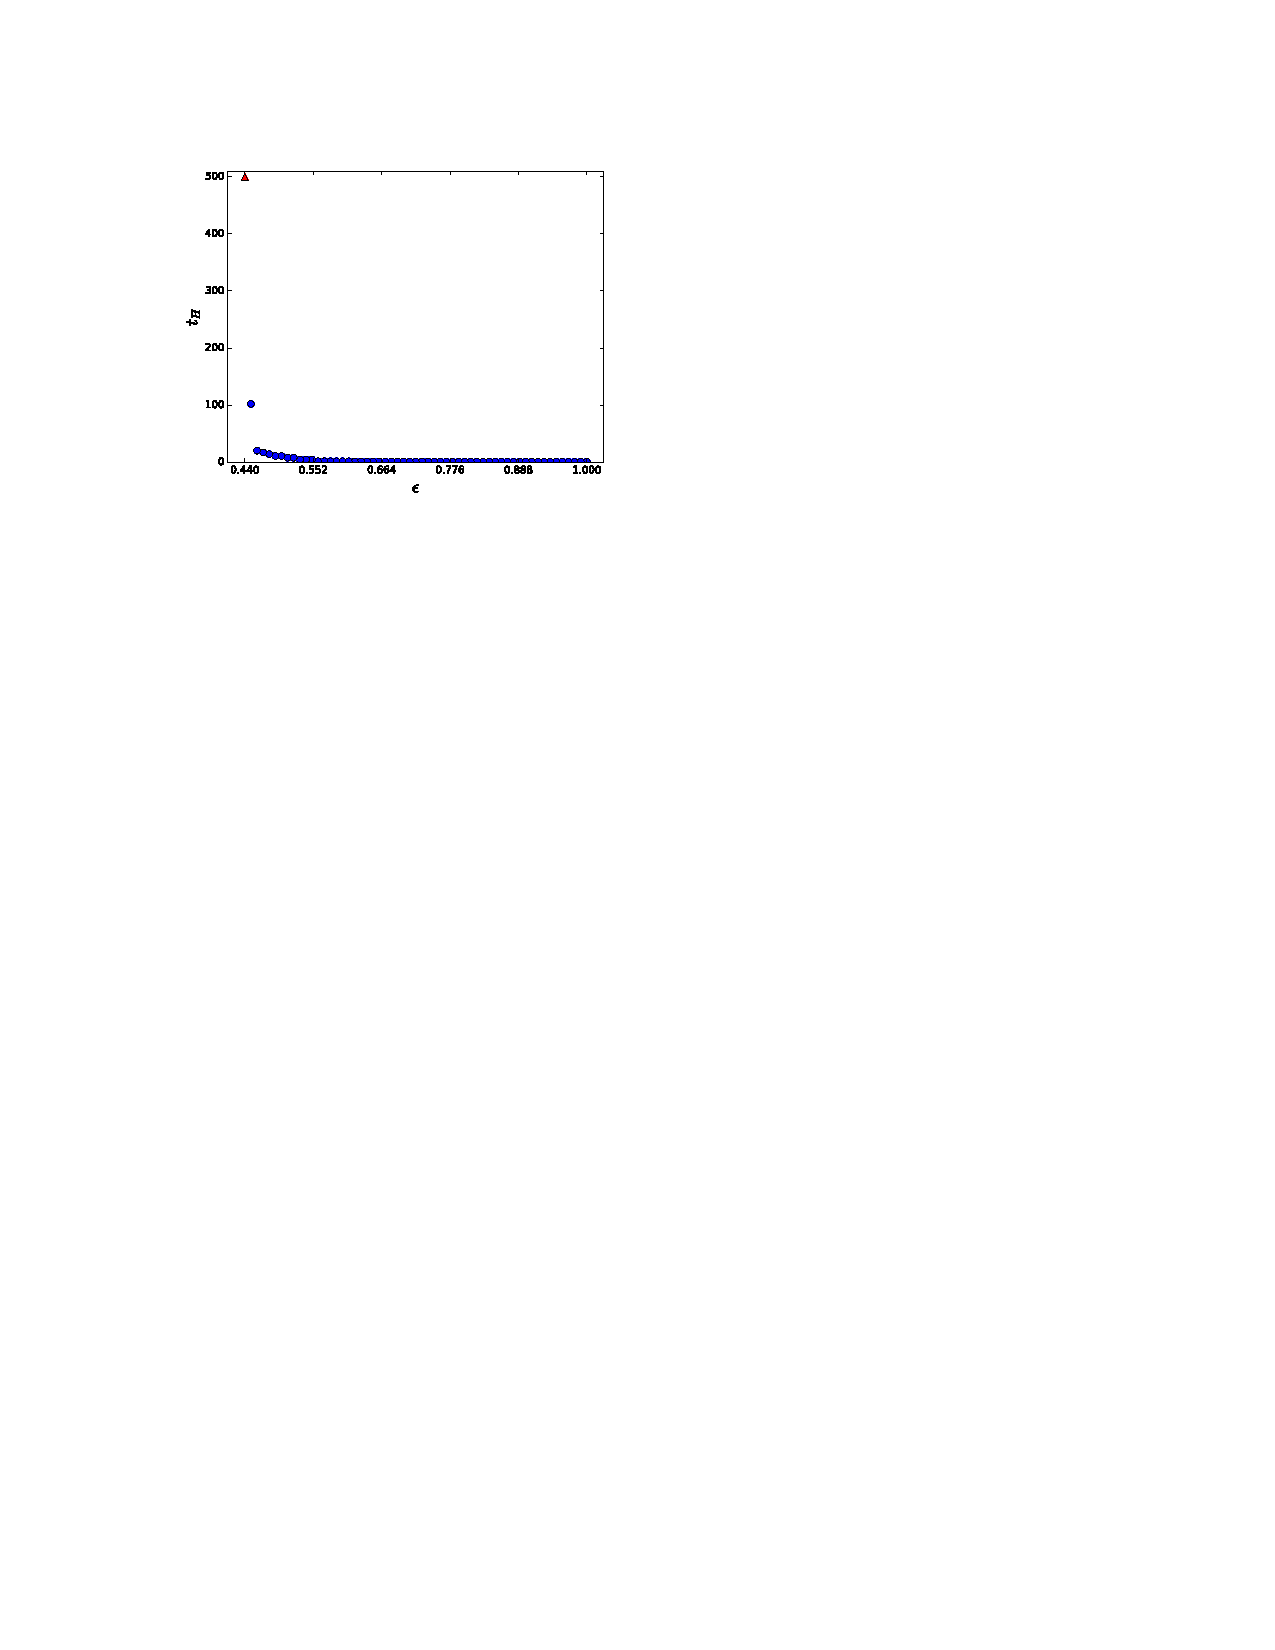
\includegraphics[scale=0.75]{m0w15} \\ $\mu =0$, $\sigma =1.5$
    \end{figure}
  \column{0.5\textwidth}
    \begin{figure}
    \centering
    \uncover<2->{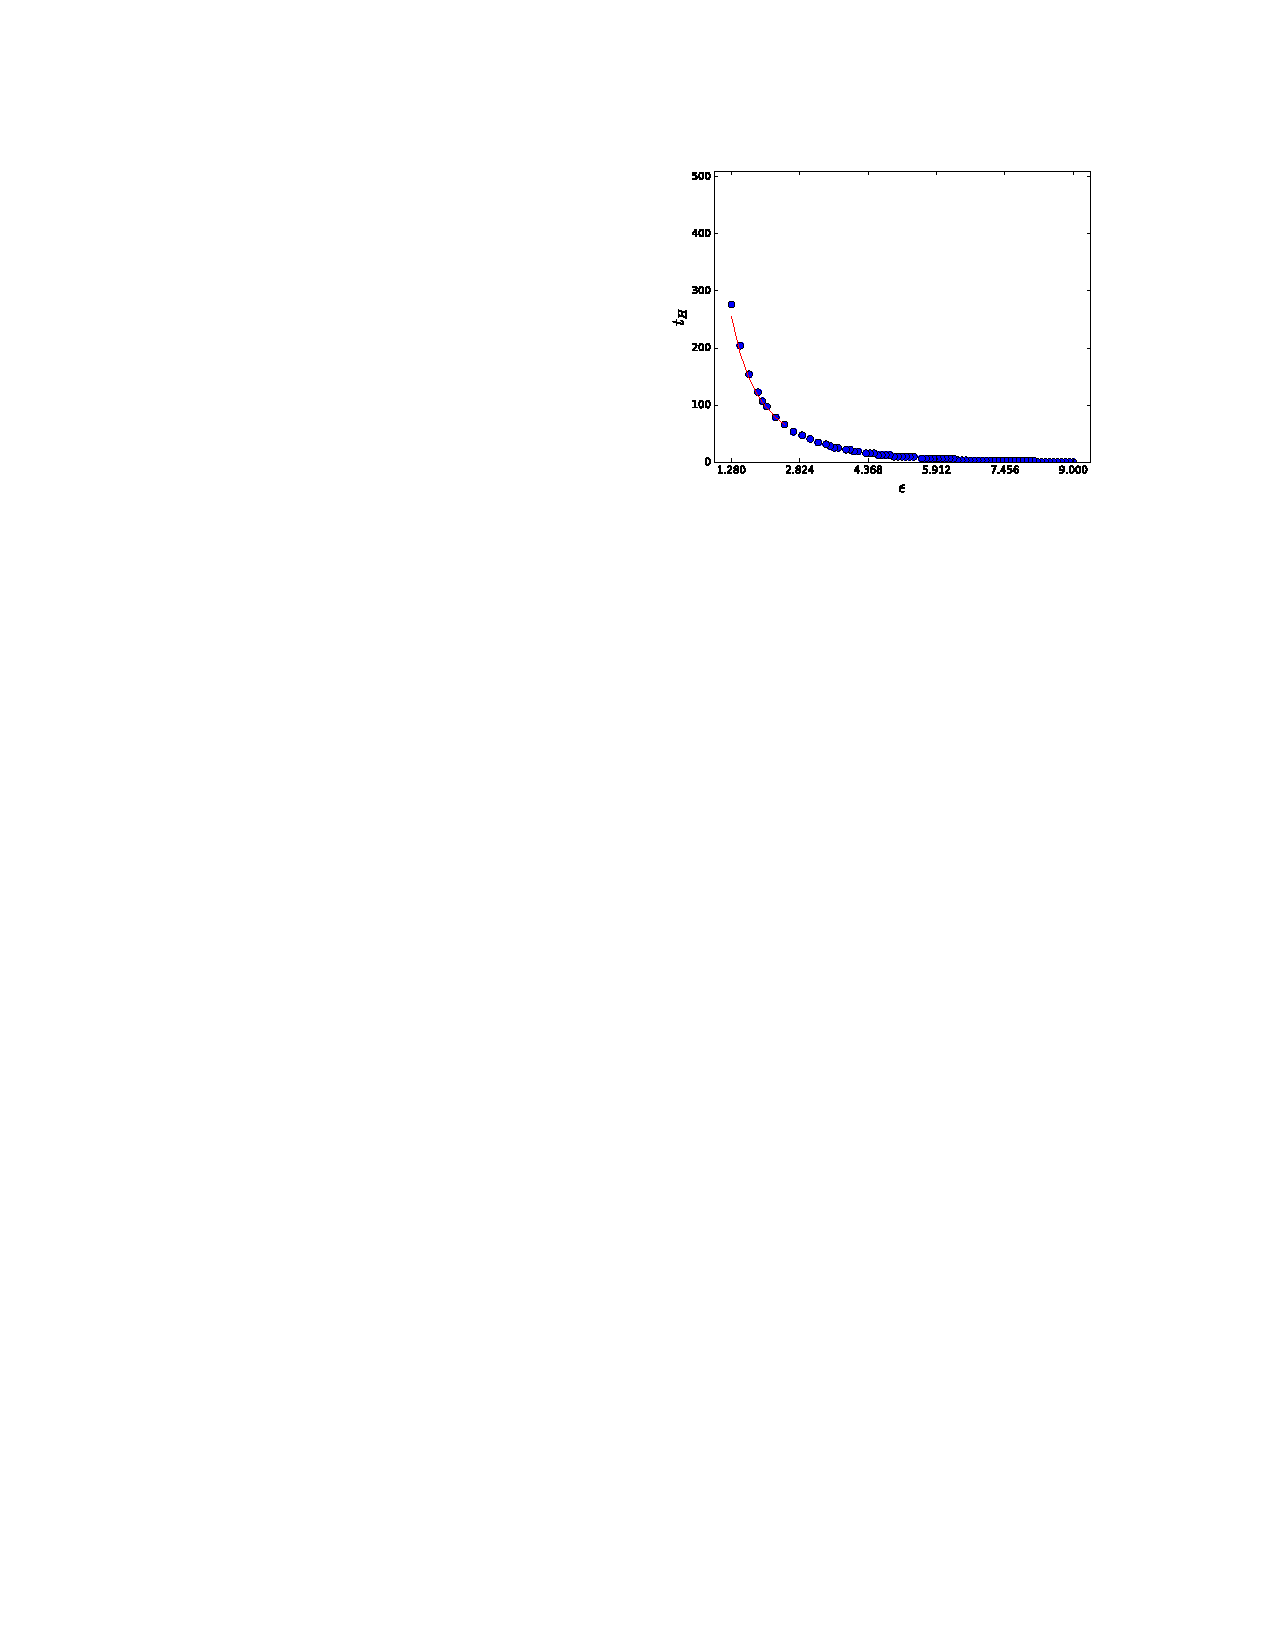
\includegraphics[scale=0.75]{m0w025} \\ $\mu = 5$, $\sigma=0.25$}
    \end{figure}
  \end{columns}
}

\frame
{
  \frametitle{Metastable Profiles}
  \bi
  \its Scaling of $p > 2$
  \ei
  \begin{columns}
  \column{0.5\textwidth}
    \begin{figure}
    \centering
    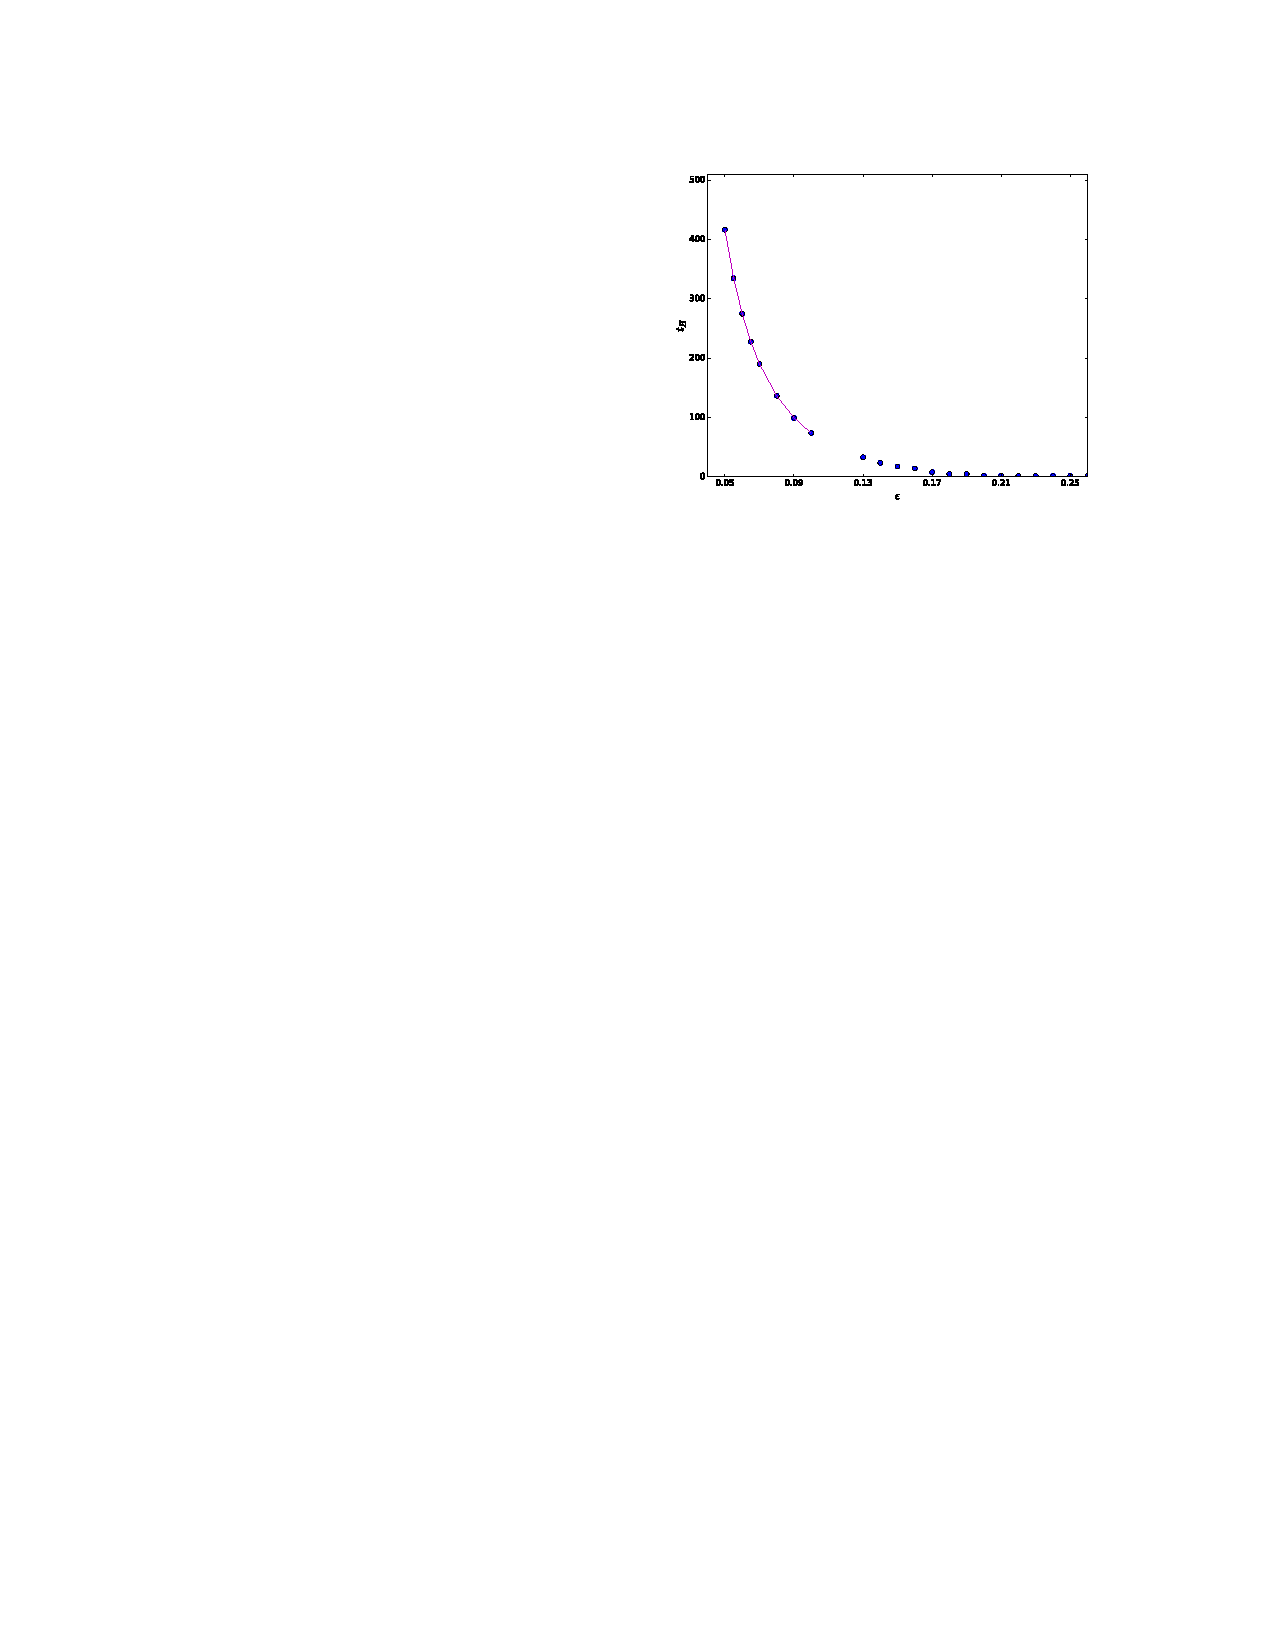
\includegraphics[scale=0.75]{m5w17} \\ $\mu = 5$, $\sigma = 1.7$
    \end{figure}
  \column{0.5\textwidth}
    \begin{figure}
    \centering
    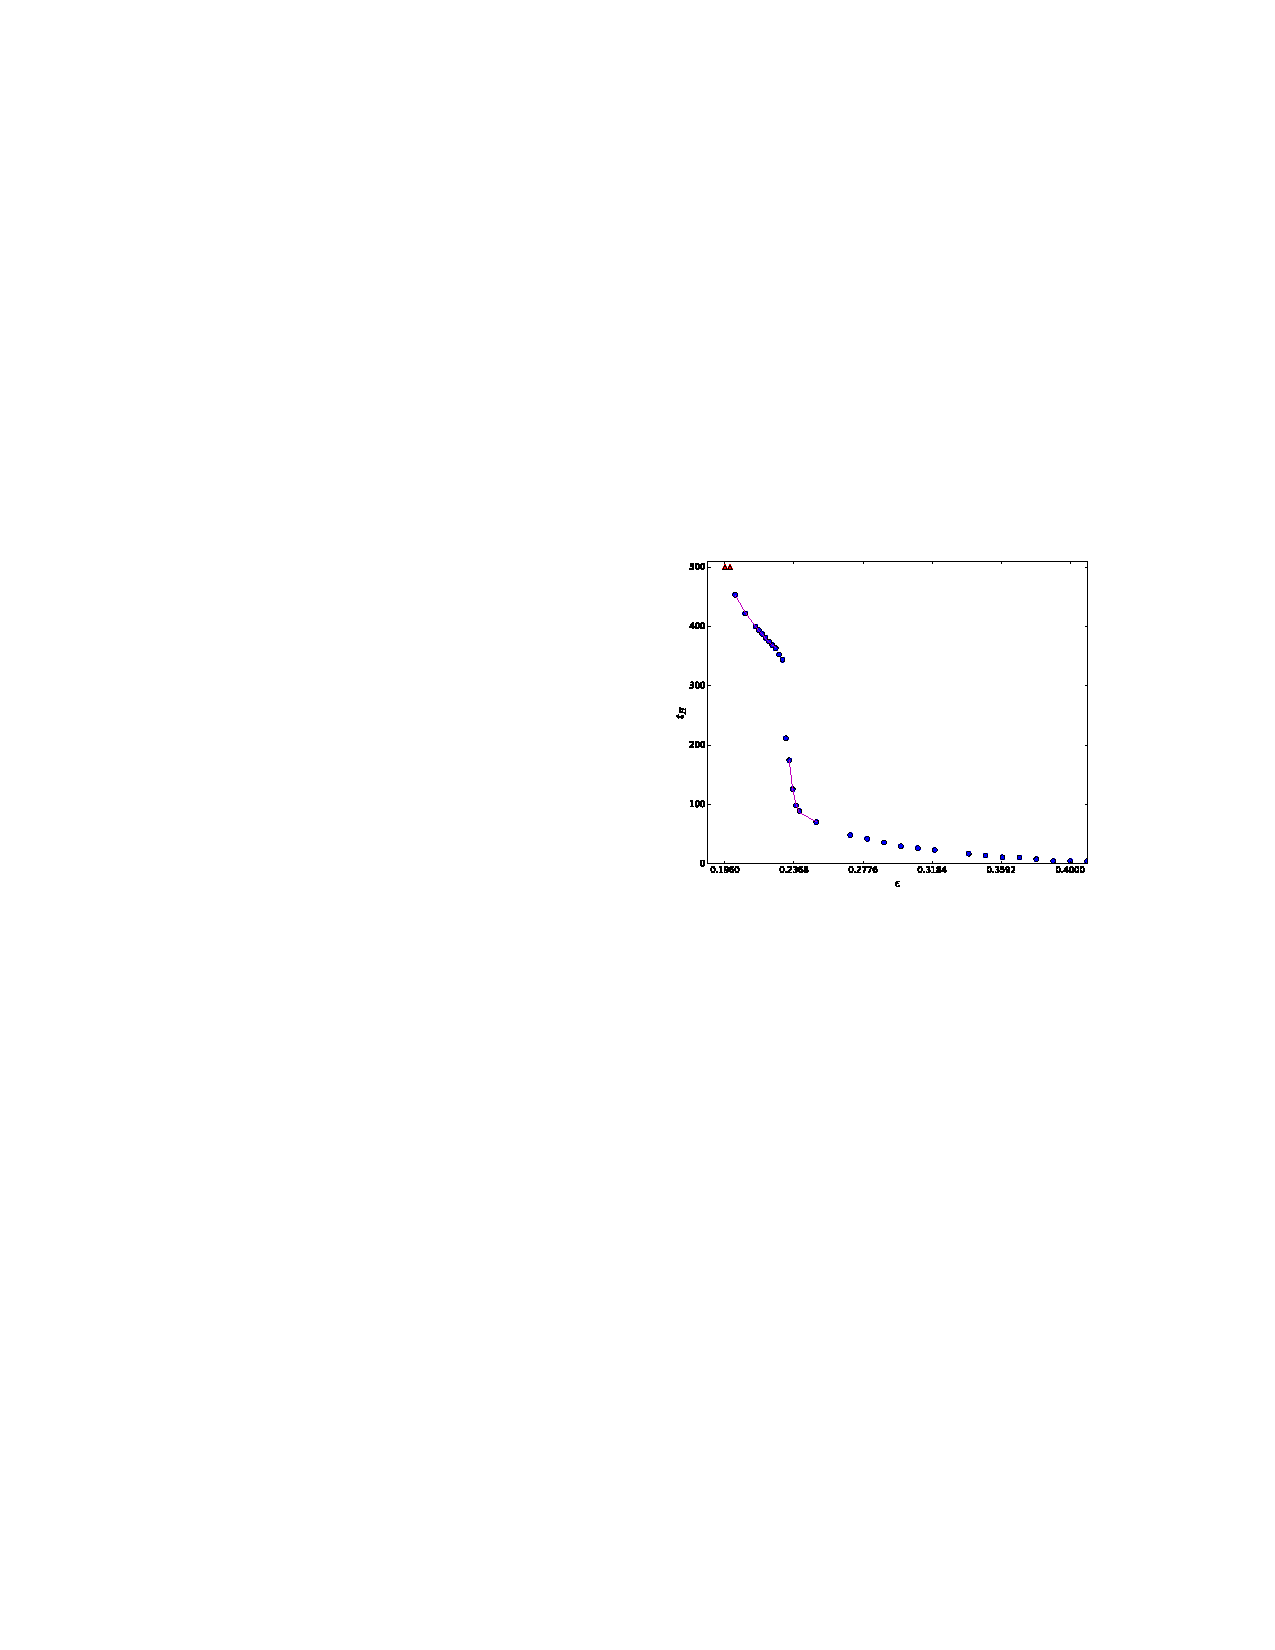
\includegraphics[scale=0.75]{m05w17} \\ $\mu = 0.5$, $\sigma = 1.7$
    \end{figure}
  \end{columns}
}

\frame
{
  \frametitle{Irregular Profiles I}
  \bi
  \its No scaling
  \ei
  \begin{columns}
  \column{0.45\textwidth}
  	\begin{figure}
  	\centering
  	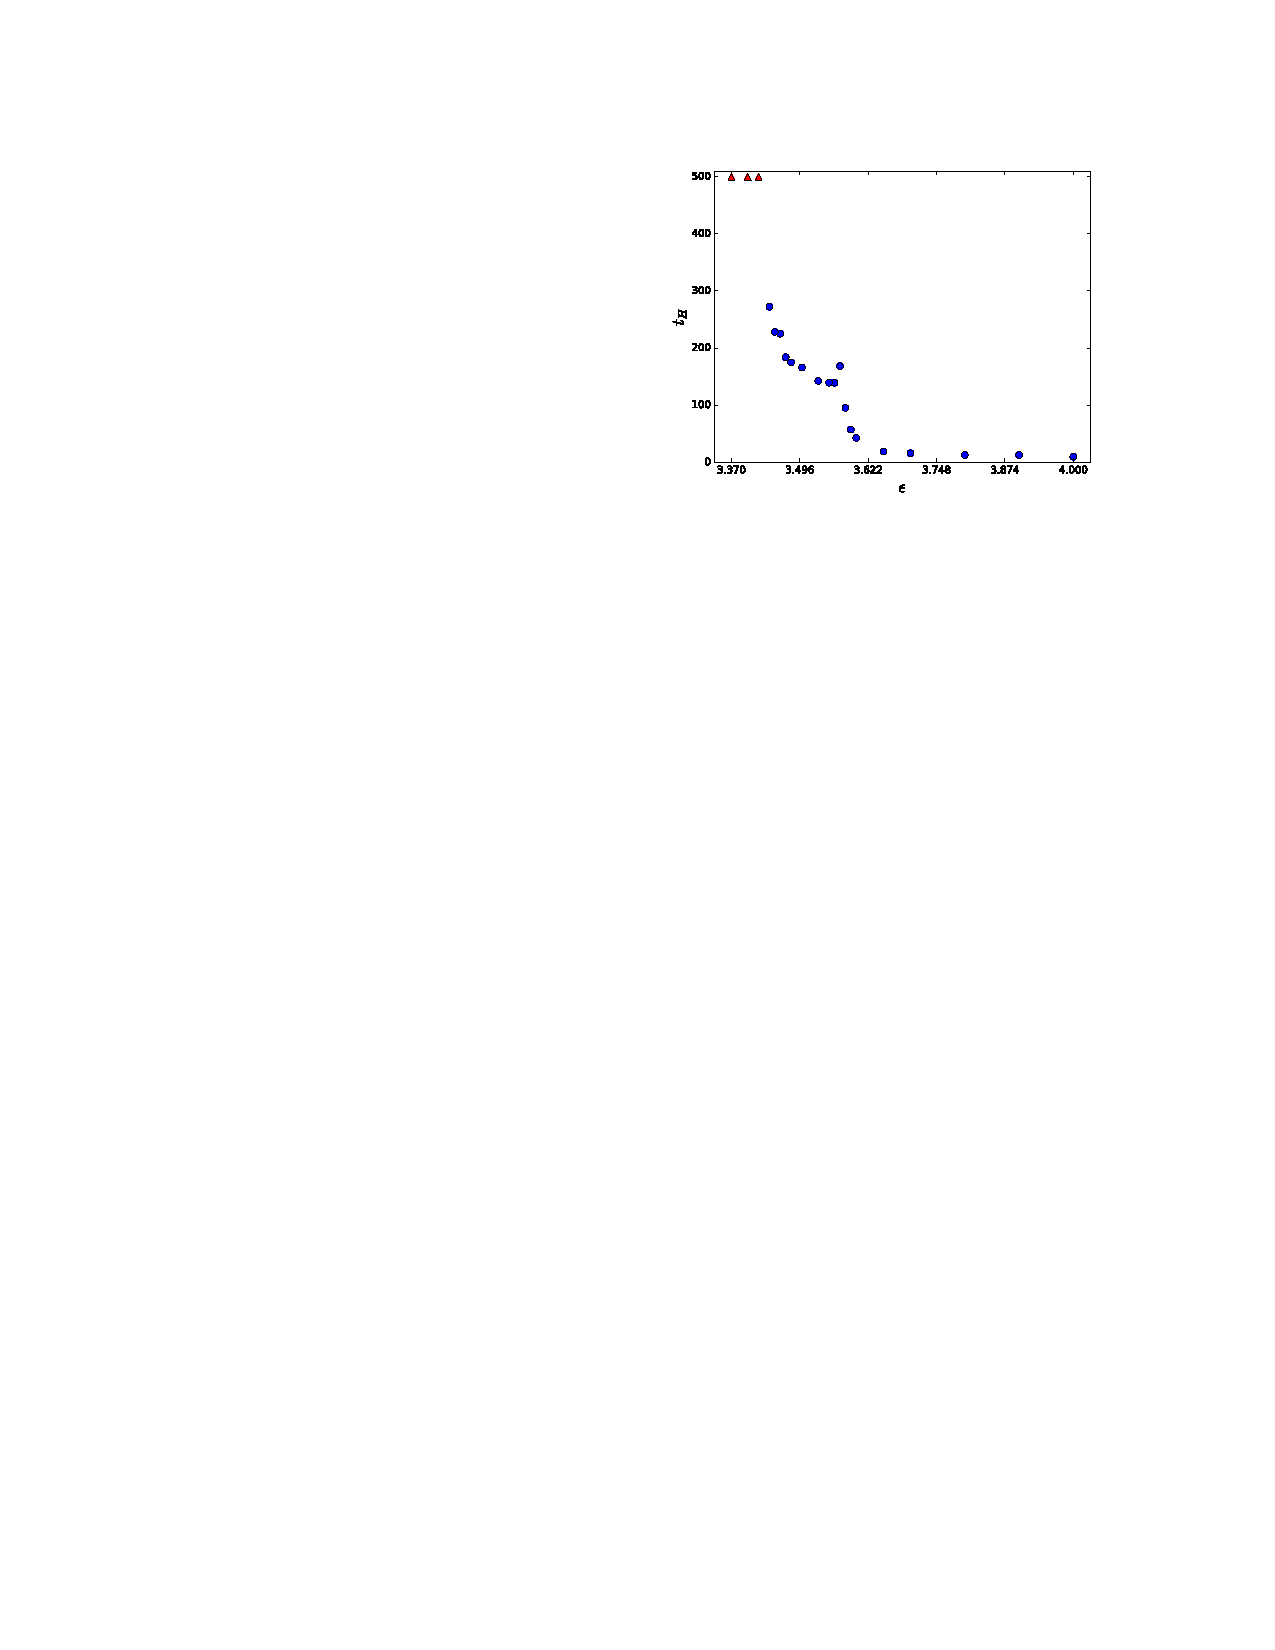
\includegraphics[width=\textwidth]{m5w034} \\ $\mu = 5$, $\sigma = 0.34$
  	\end{figure}
  \column{0.45\textwidth}
  	\begin{figure}
	\centering
	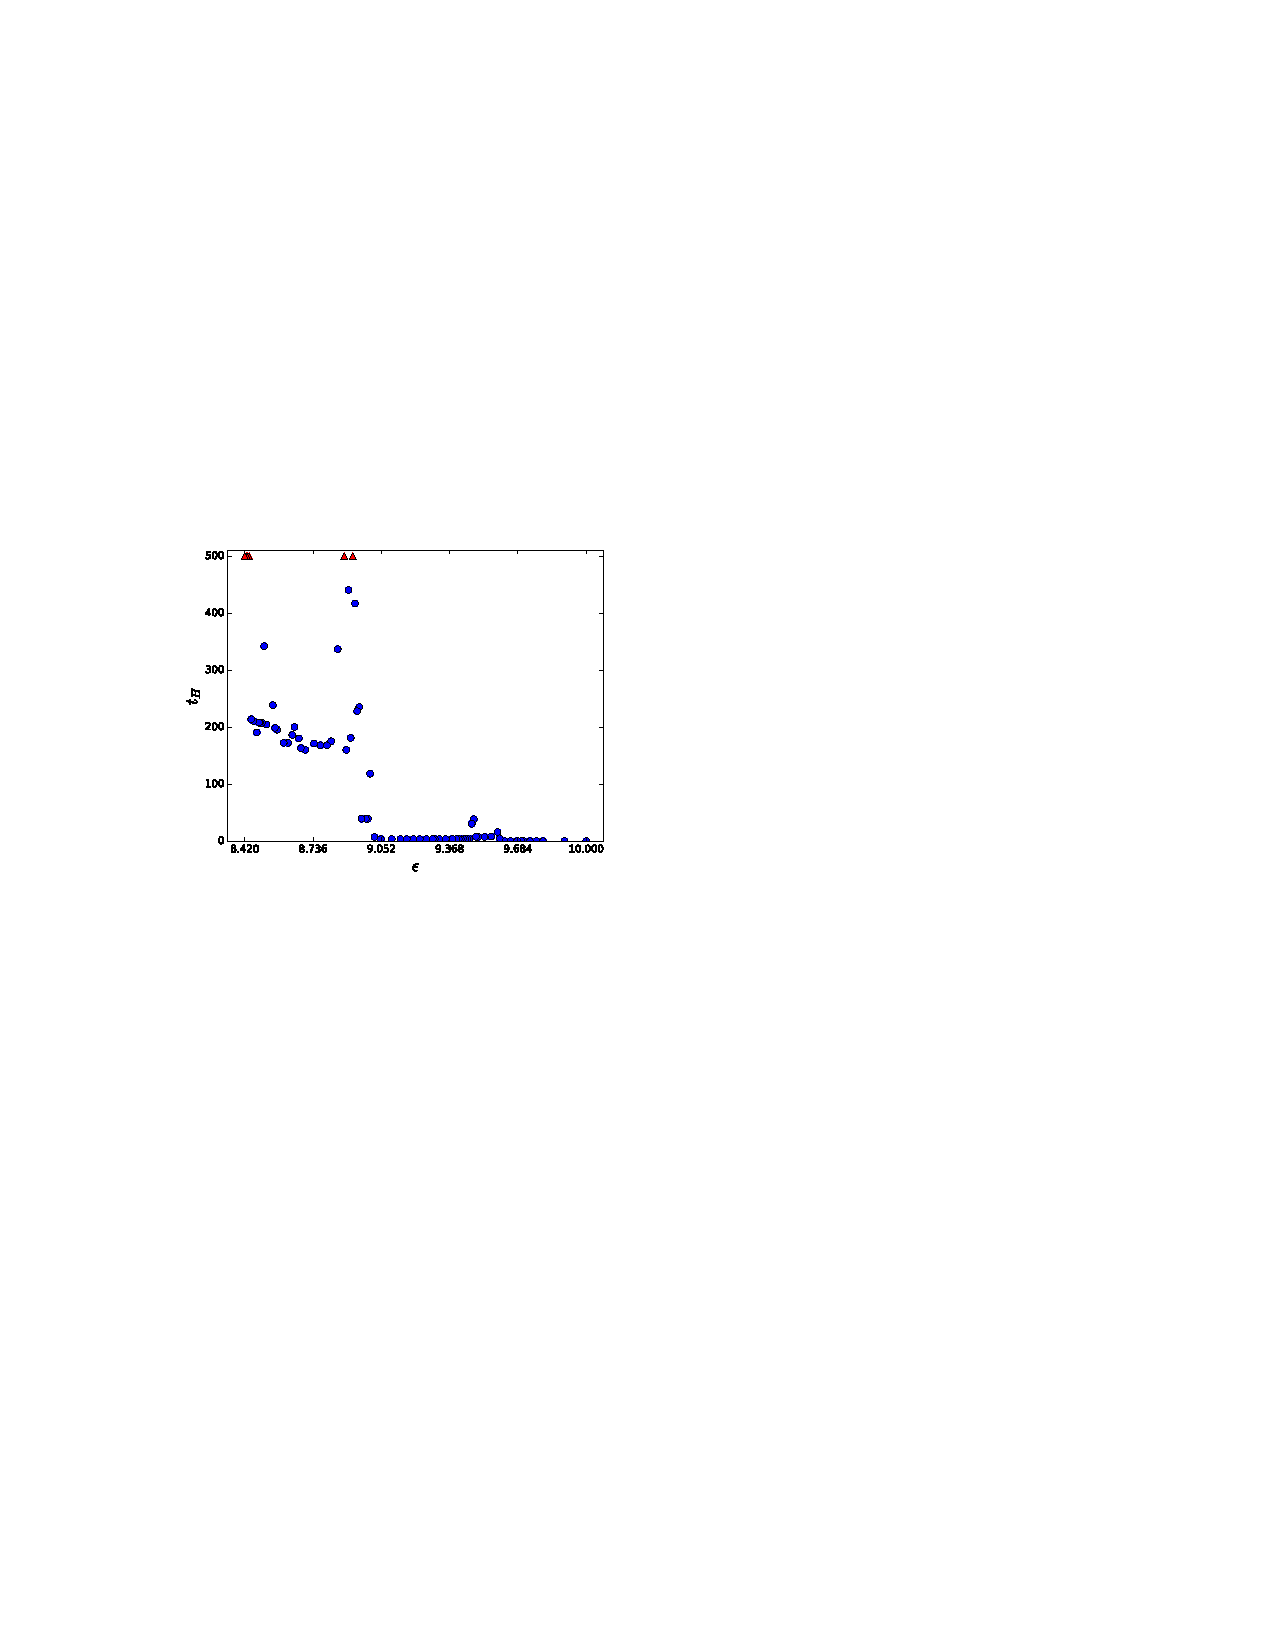
\includegraphics[width=\textwidth]{m20w016} \\ $\mu = 20$, $\sigma = 0.16$
  	\end{figure}
  \end{columns}
}

\frame
{
  \frametitle{Irregular Profiles II}
  \bi
  \its Evidence of chaotic behaviour $\to$ possible self-interaction
  \its Previous chaotic evolution only seen in thin-shell interactions\footnotemark\ in AdS, scalar collapse in Gauss-Bonnet gravity\footnotemark
  \ei
  \vspace{-0.15in}
  \begin{columns}
    \column{0.75\textwidth}
      \begin{figure}
  	\centering
	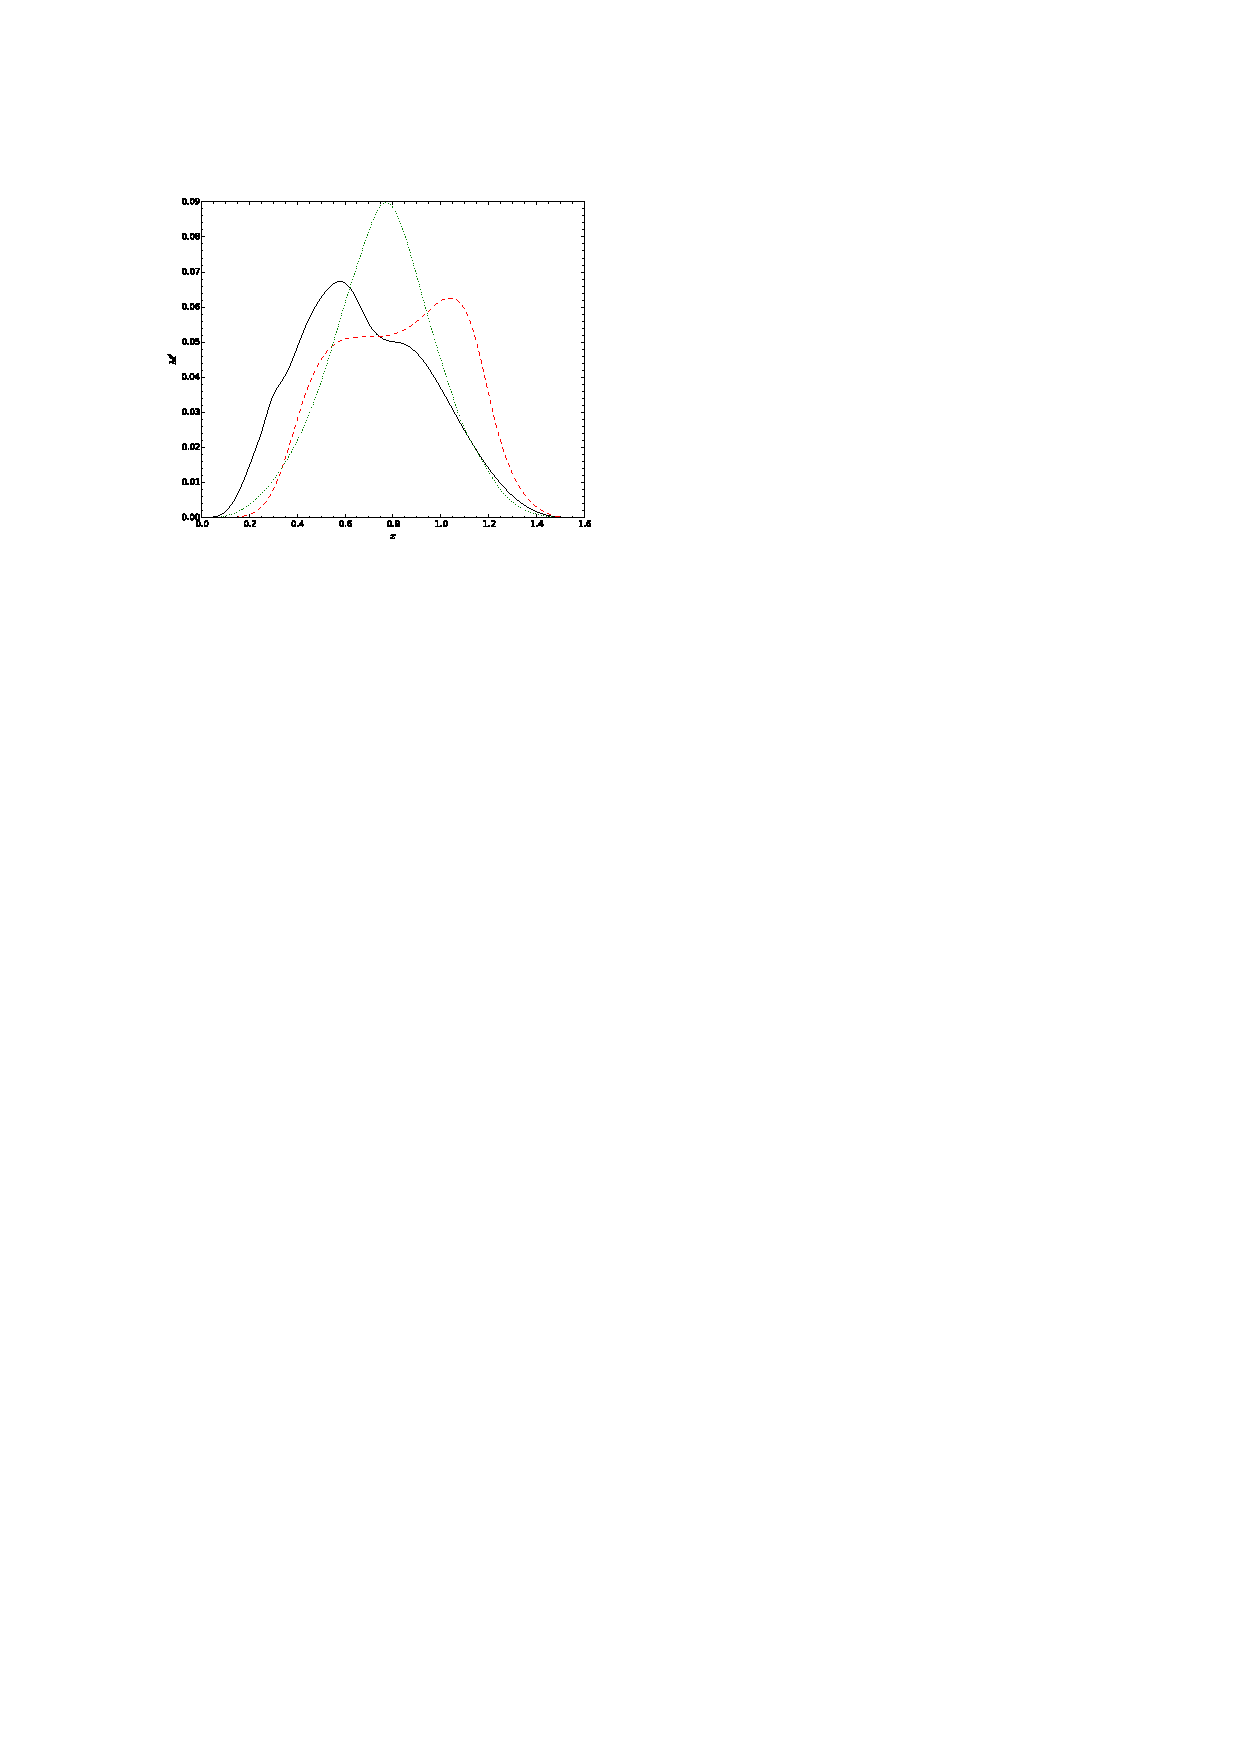
\includegraphics[scale=0.75]{selfinteraction} \\ $\mu = 0$, $\sigma=1.1$, $\epsilon = 1.01$
       \end{figure}
    \column{0.25\textwidth}
    \hspace{-0.6in}
       $t = 60, {\color[rgb]{0.06,0.64,0.01} 62}, {\color[rgb]{.98,0,0.04} 64}$
   \end{columns}
  
  \footnotetext[4]{{\scr Brito {\it et al.} [1602.03535]}}
  \footnotetext[5]{{\scr Deppe, Kolly, {\it et al.} [1608.05402]}}
}

%%%%%%%%%%%%%%%%%%%%%%%%%%%%%%%%%%%%%%%%%%%%%%

\subsection{Phase Diagram \& Energy Cascades}
\frame
{
  \frametitle{Phase Diagram}
  \bi
  \its<2->{{\color{orange} Unstable}\uncover<3->{, {\color[rgb]{.34,.69,0.29} metastable}, }\uncover<4->{{\color{red} irregular}, }\uncover<5->{and {\color{blue} stable} initial data}}
  \ei 
  \begin{figure}
  \centering
  \only<1>{
  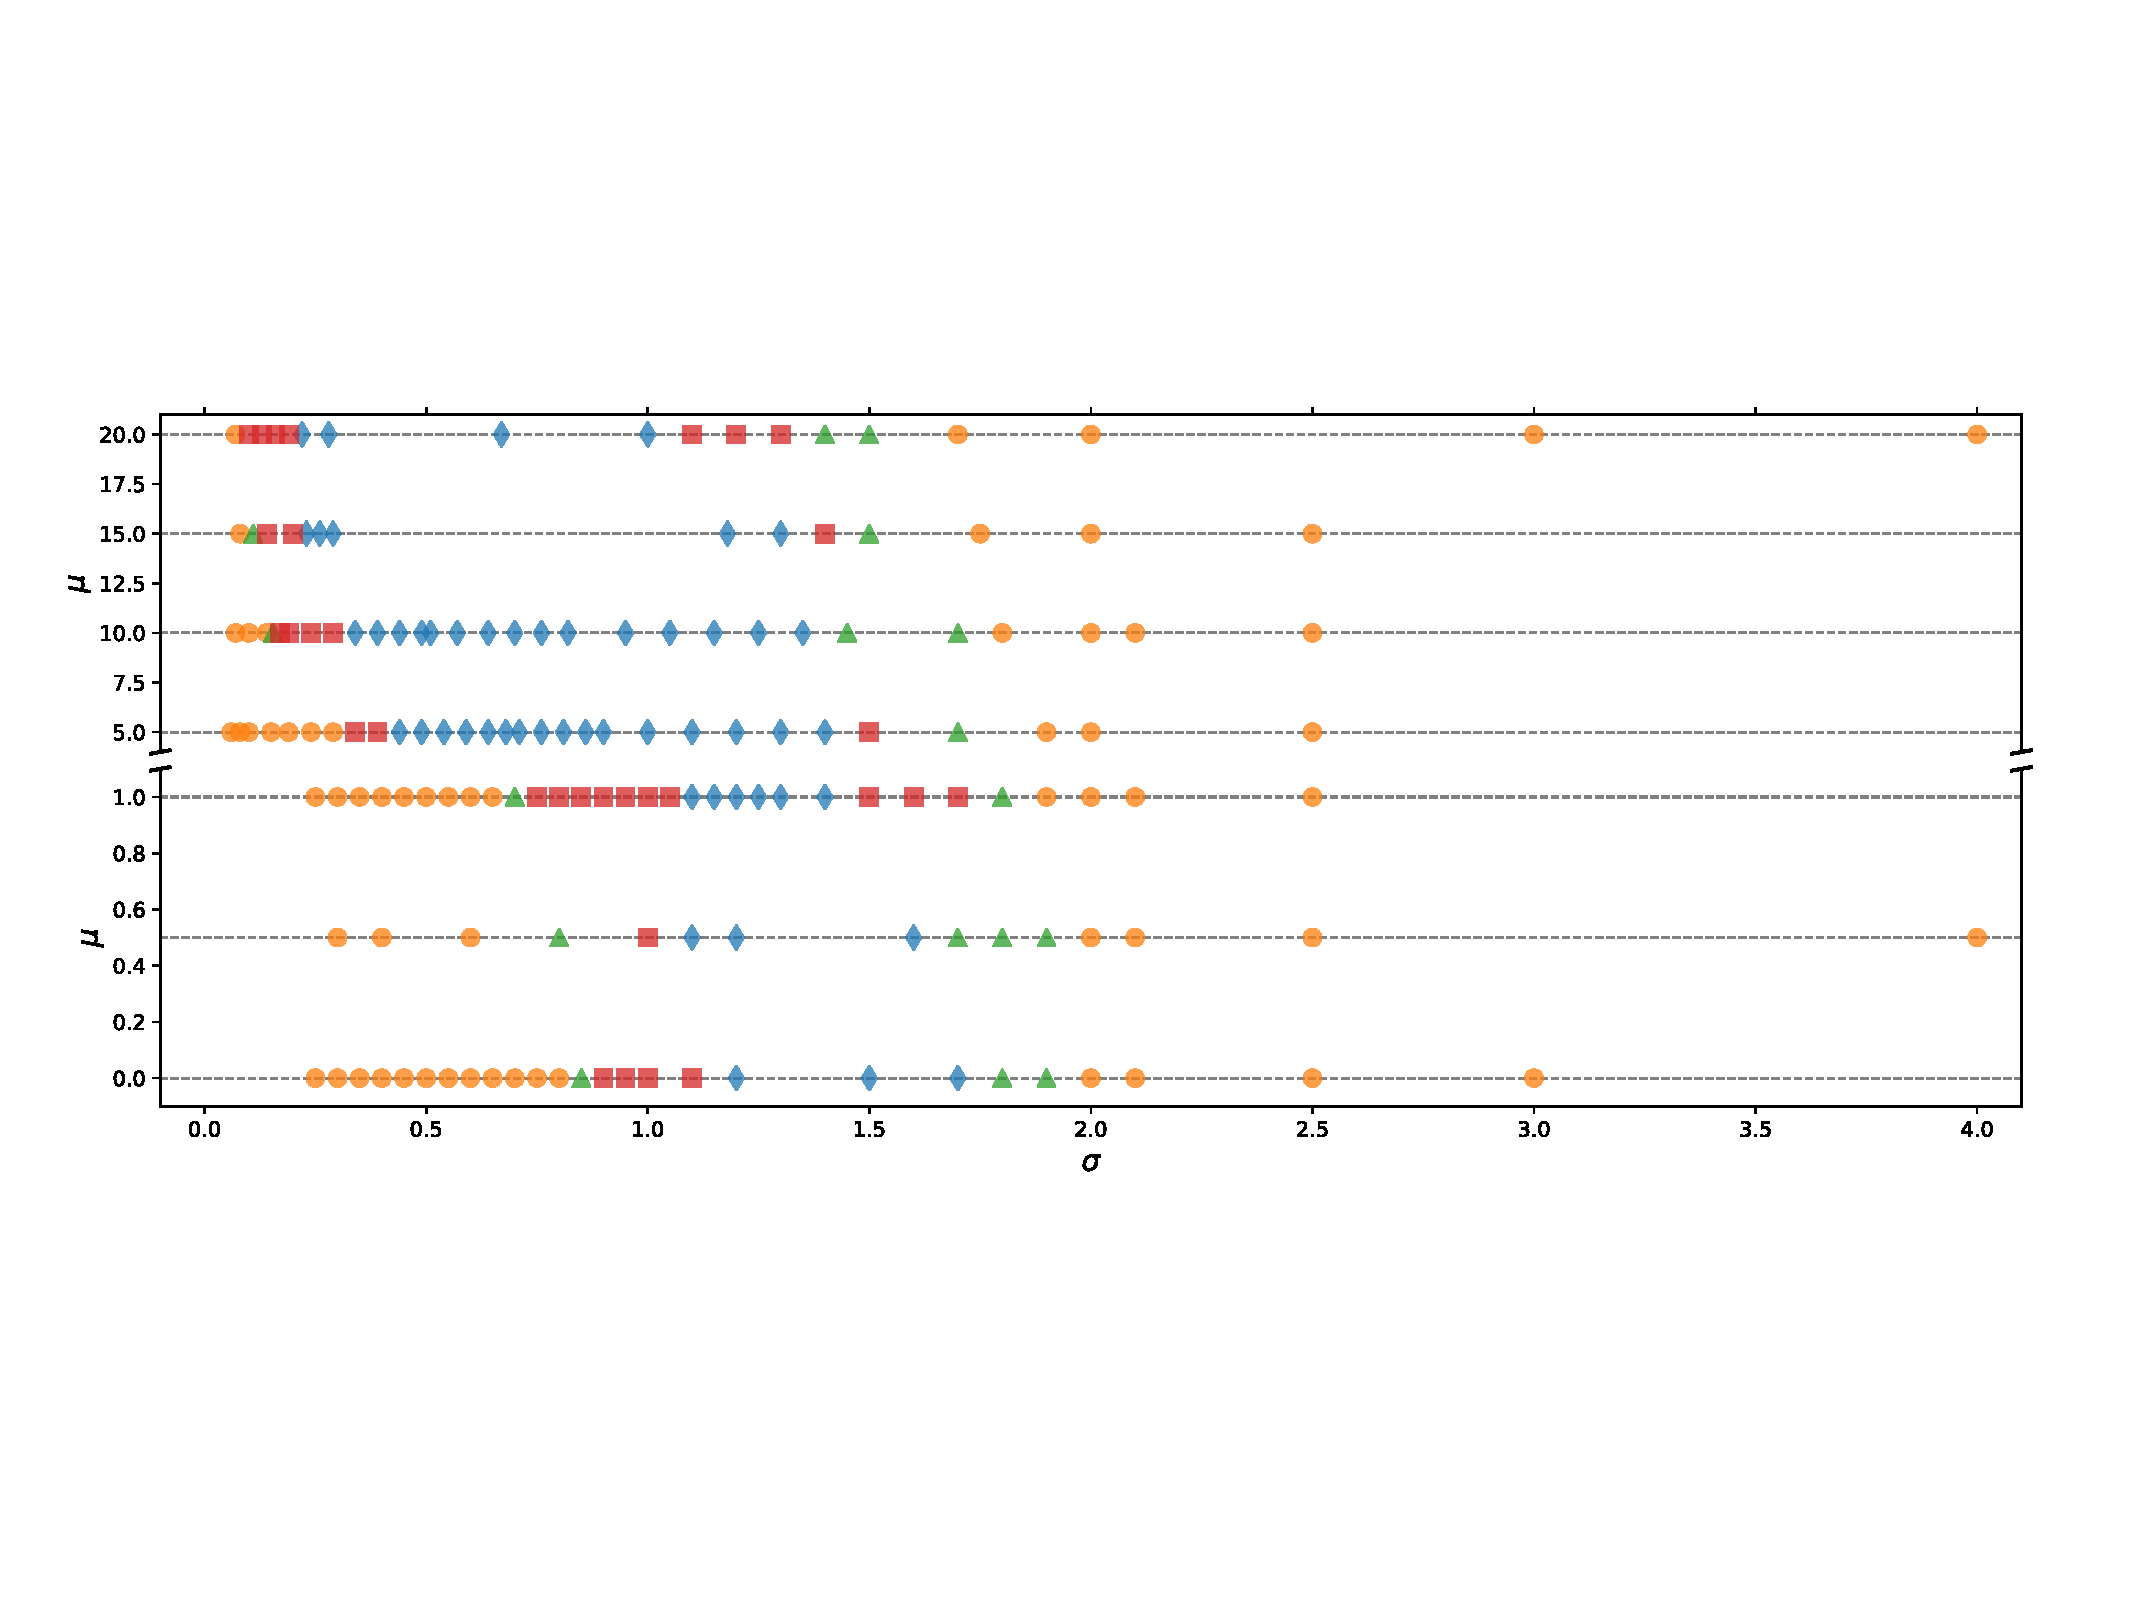
\includegraphics[width=\textwidth]{phase_plot}
  }
  \only<2>{
  \begin{center}
  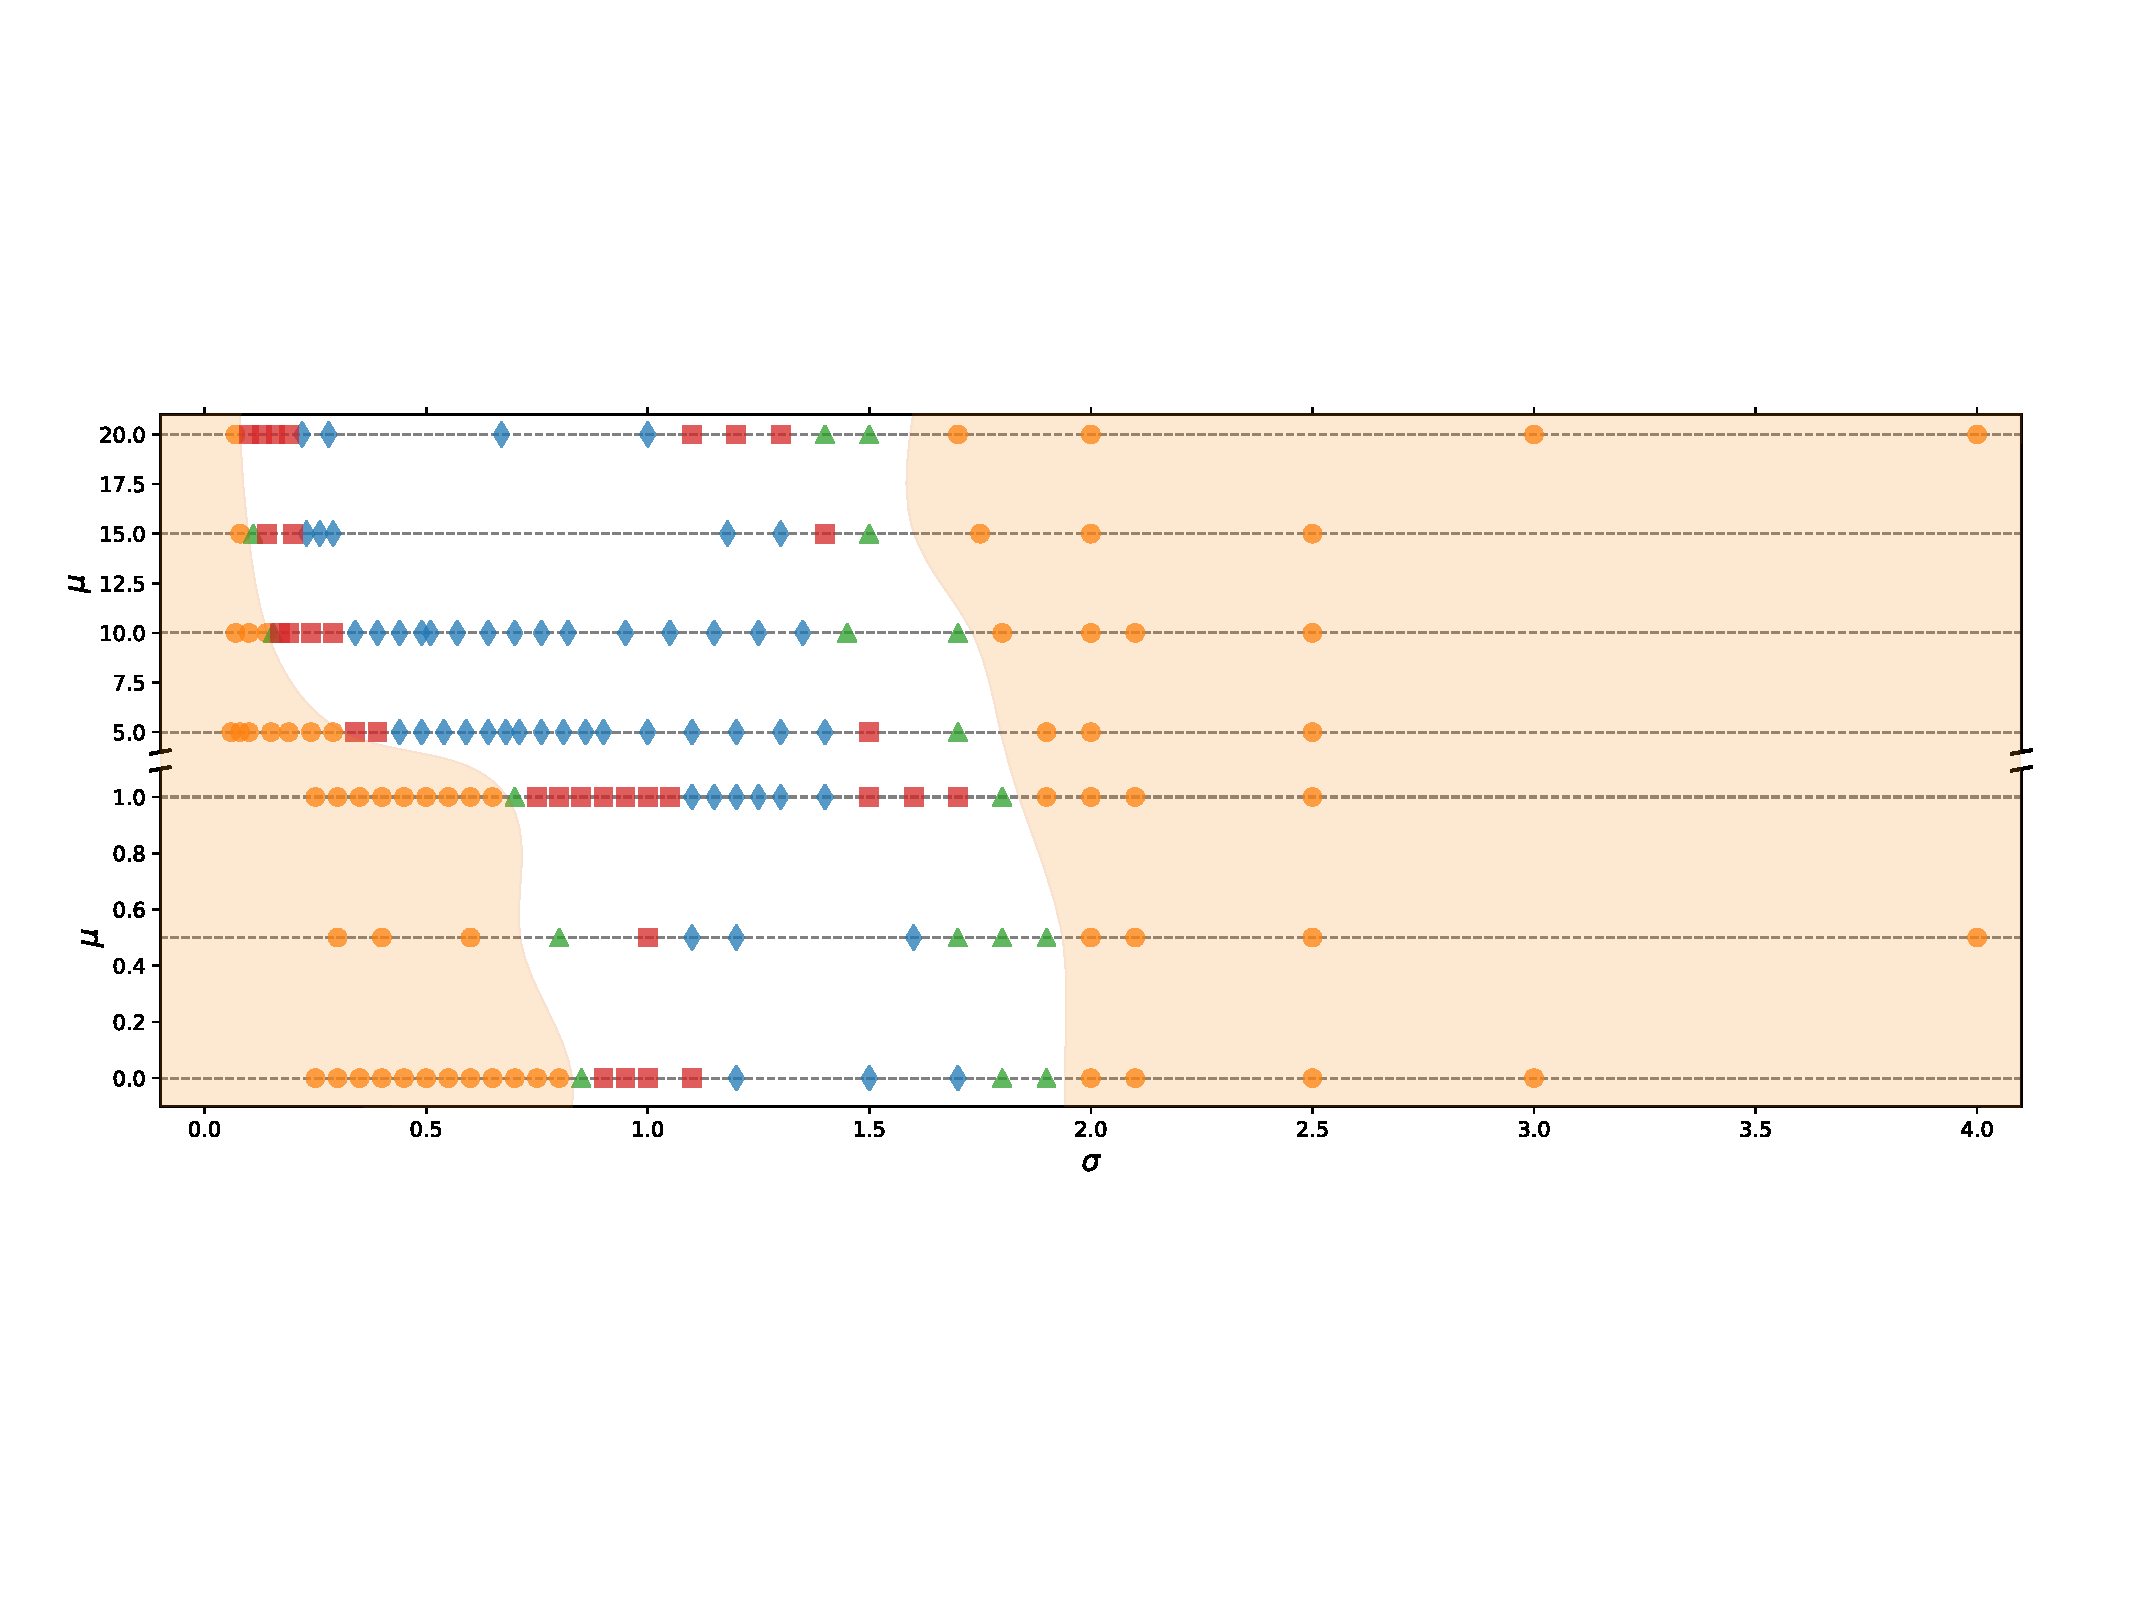
\includegraphics[width=\textwidth]{phase_sections1}
  \end{center}
  }
  \only<3>{
  \begin{center}
  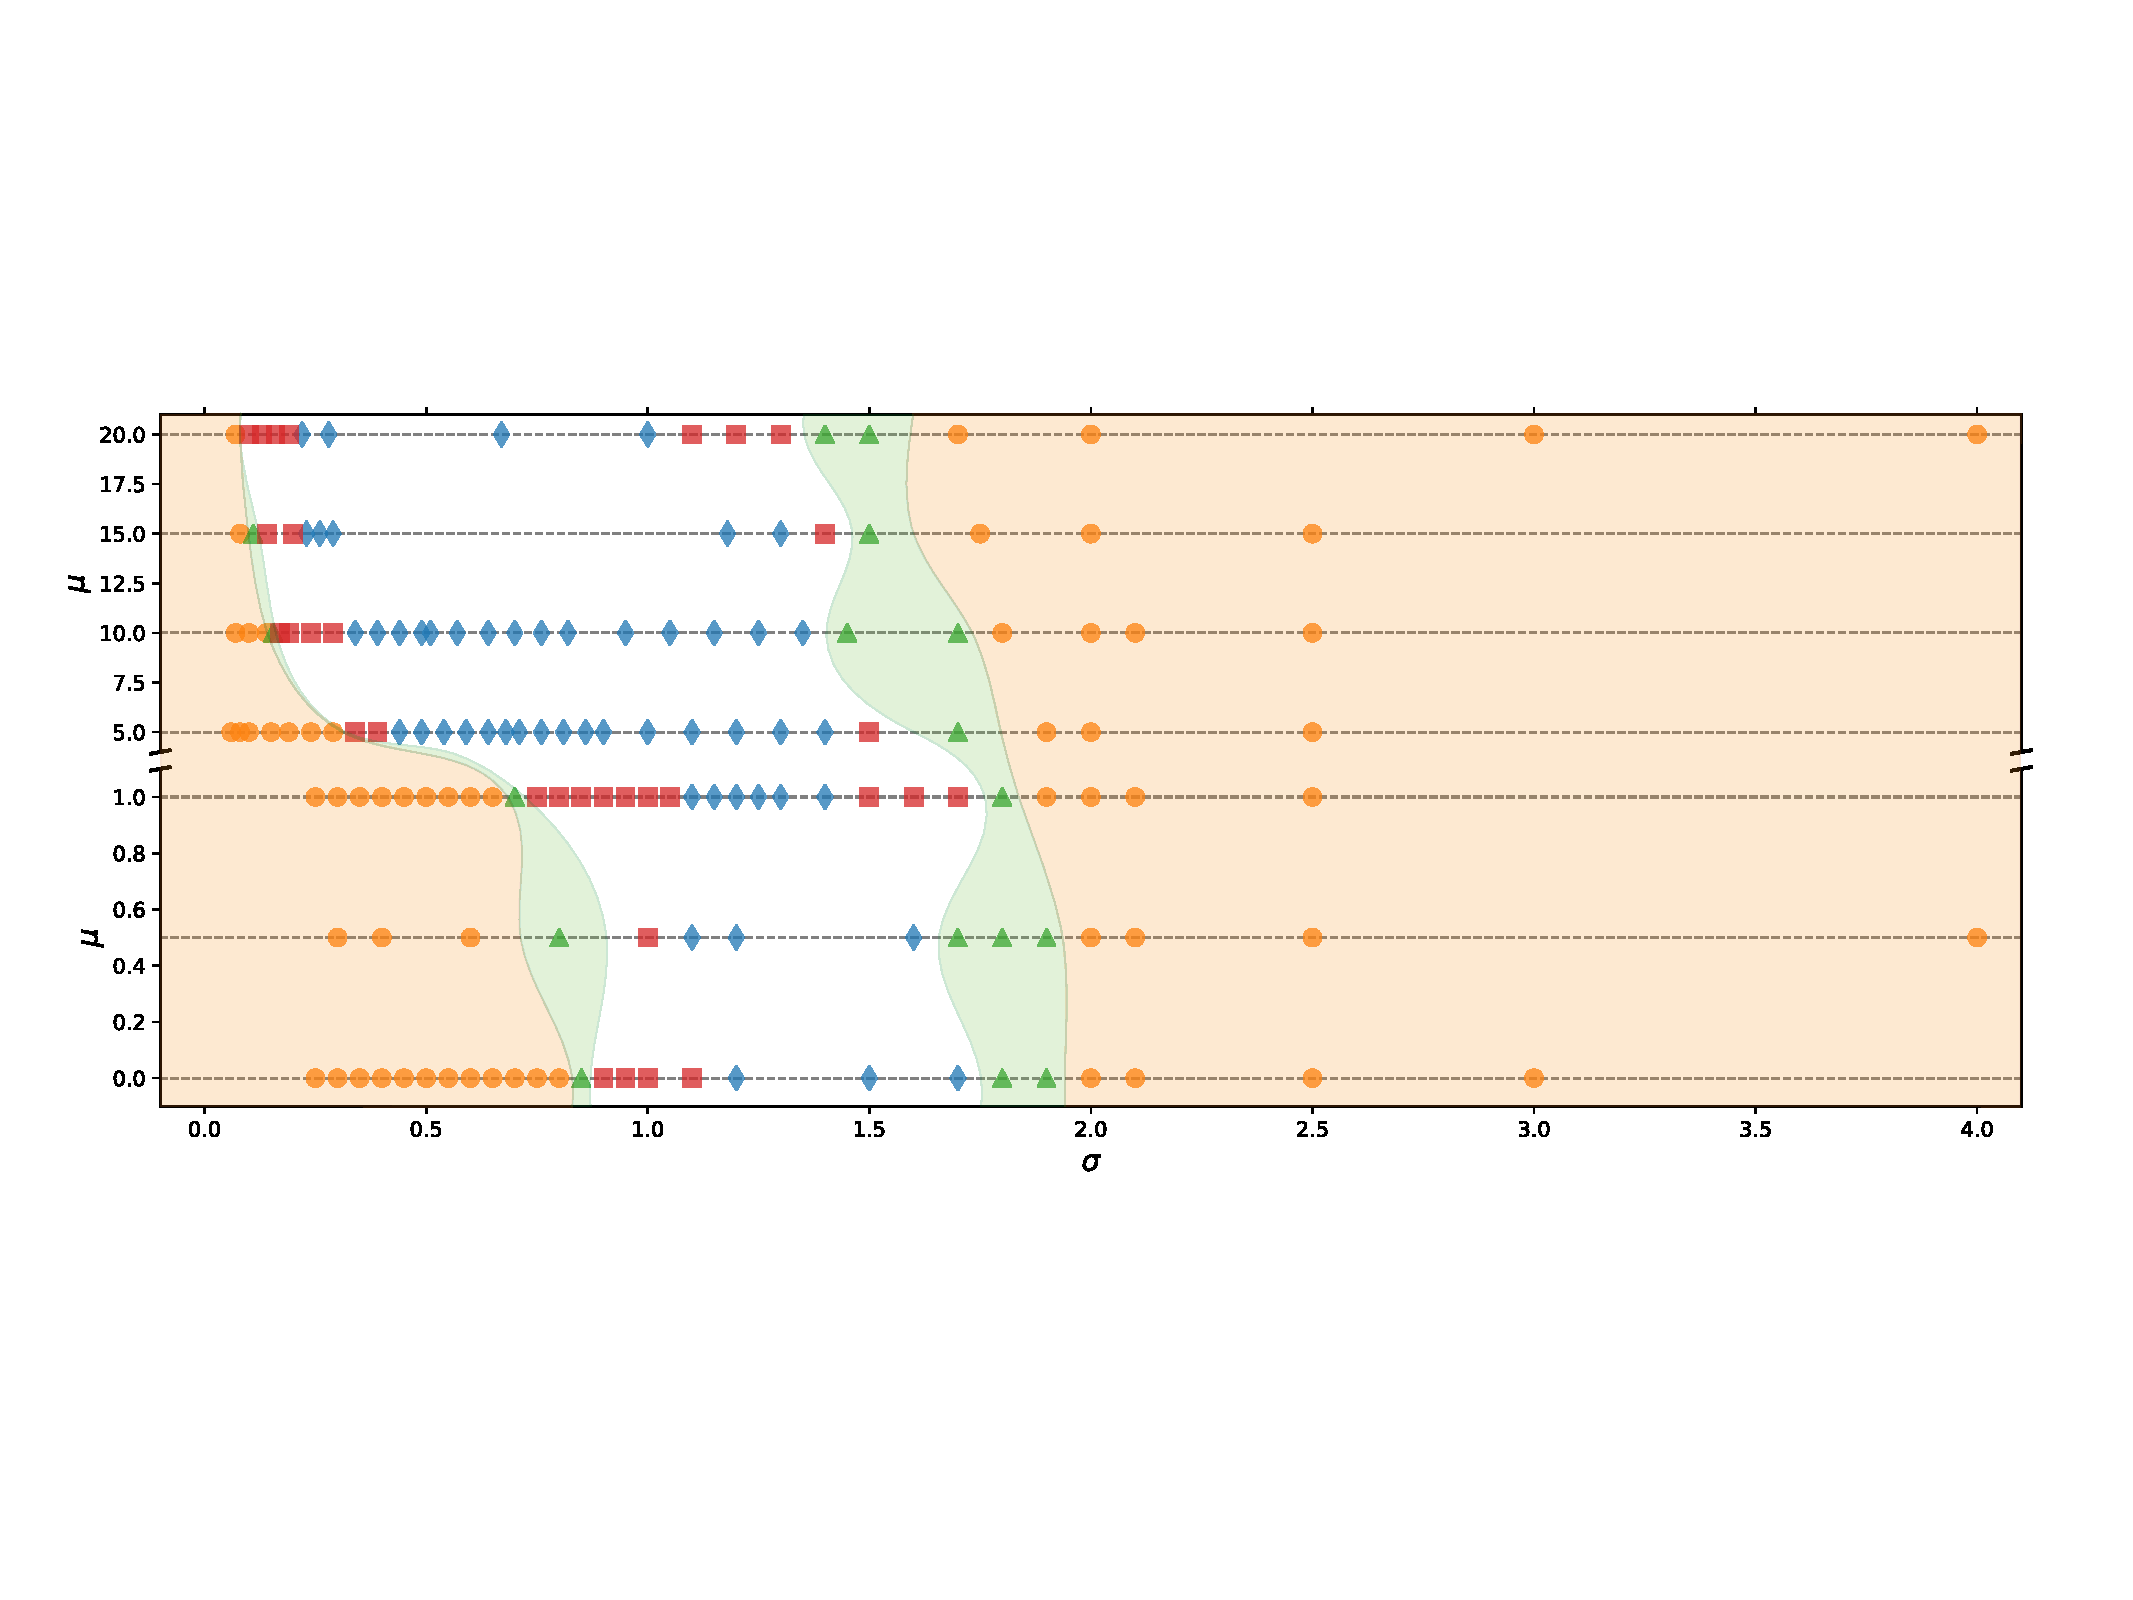
\includegraphics[width=\textwidth]{phase_sections2}
  \end{center}
  }
\only<4>{
  \begin{center}
  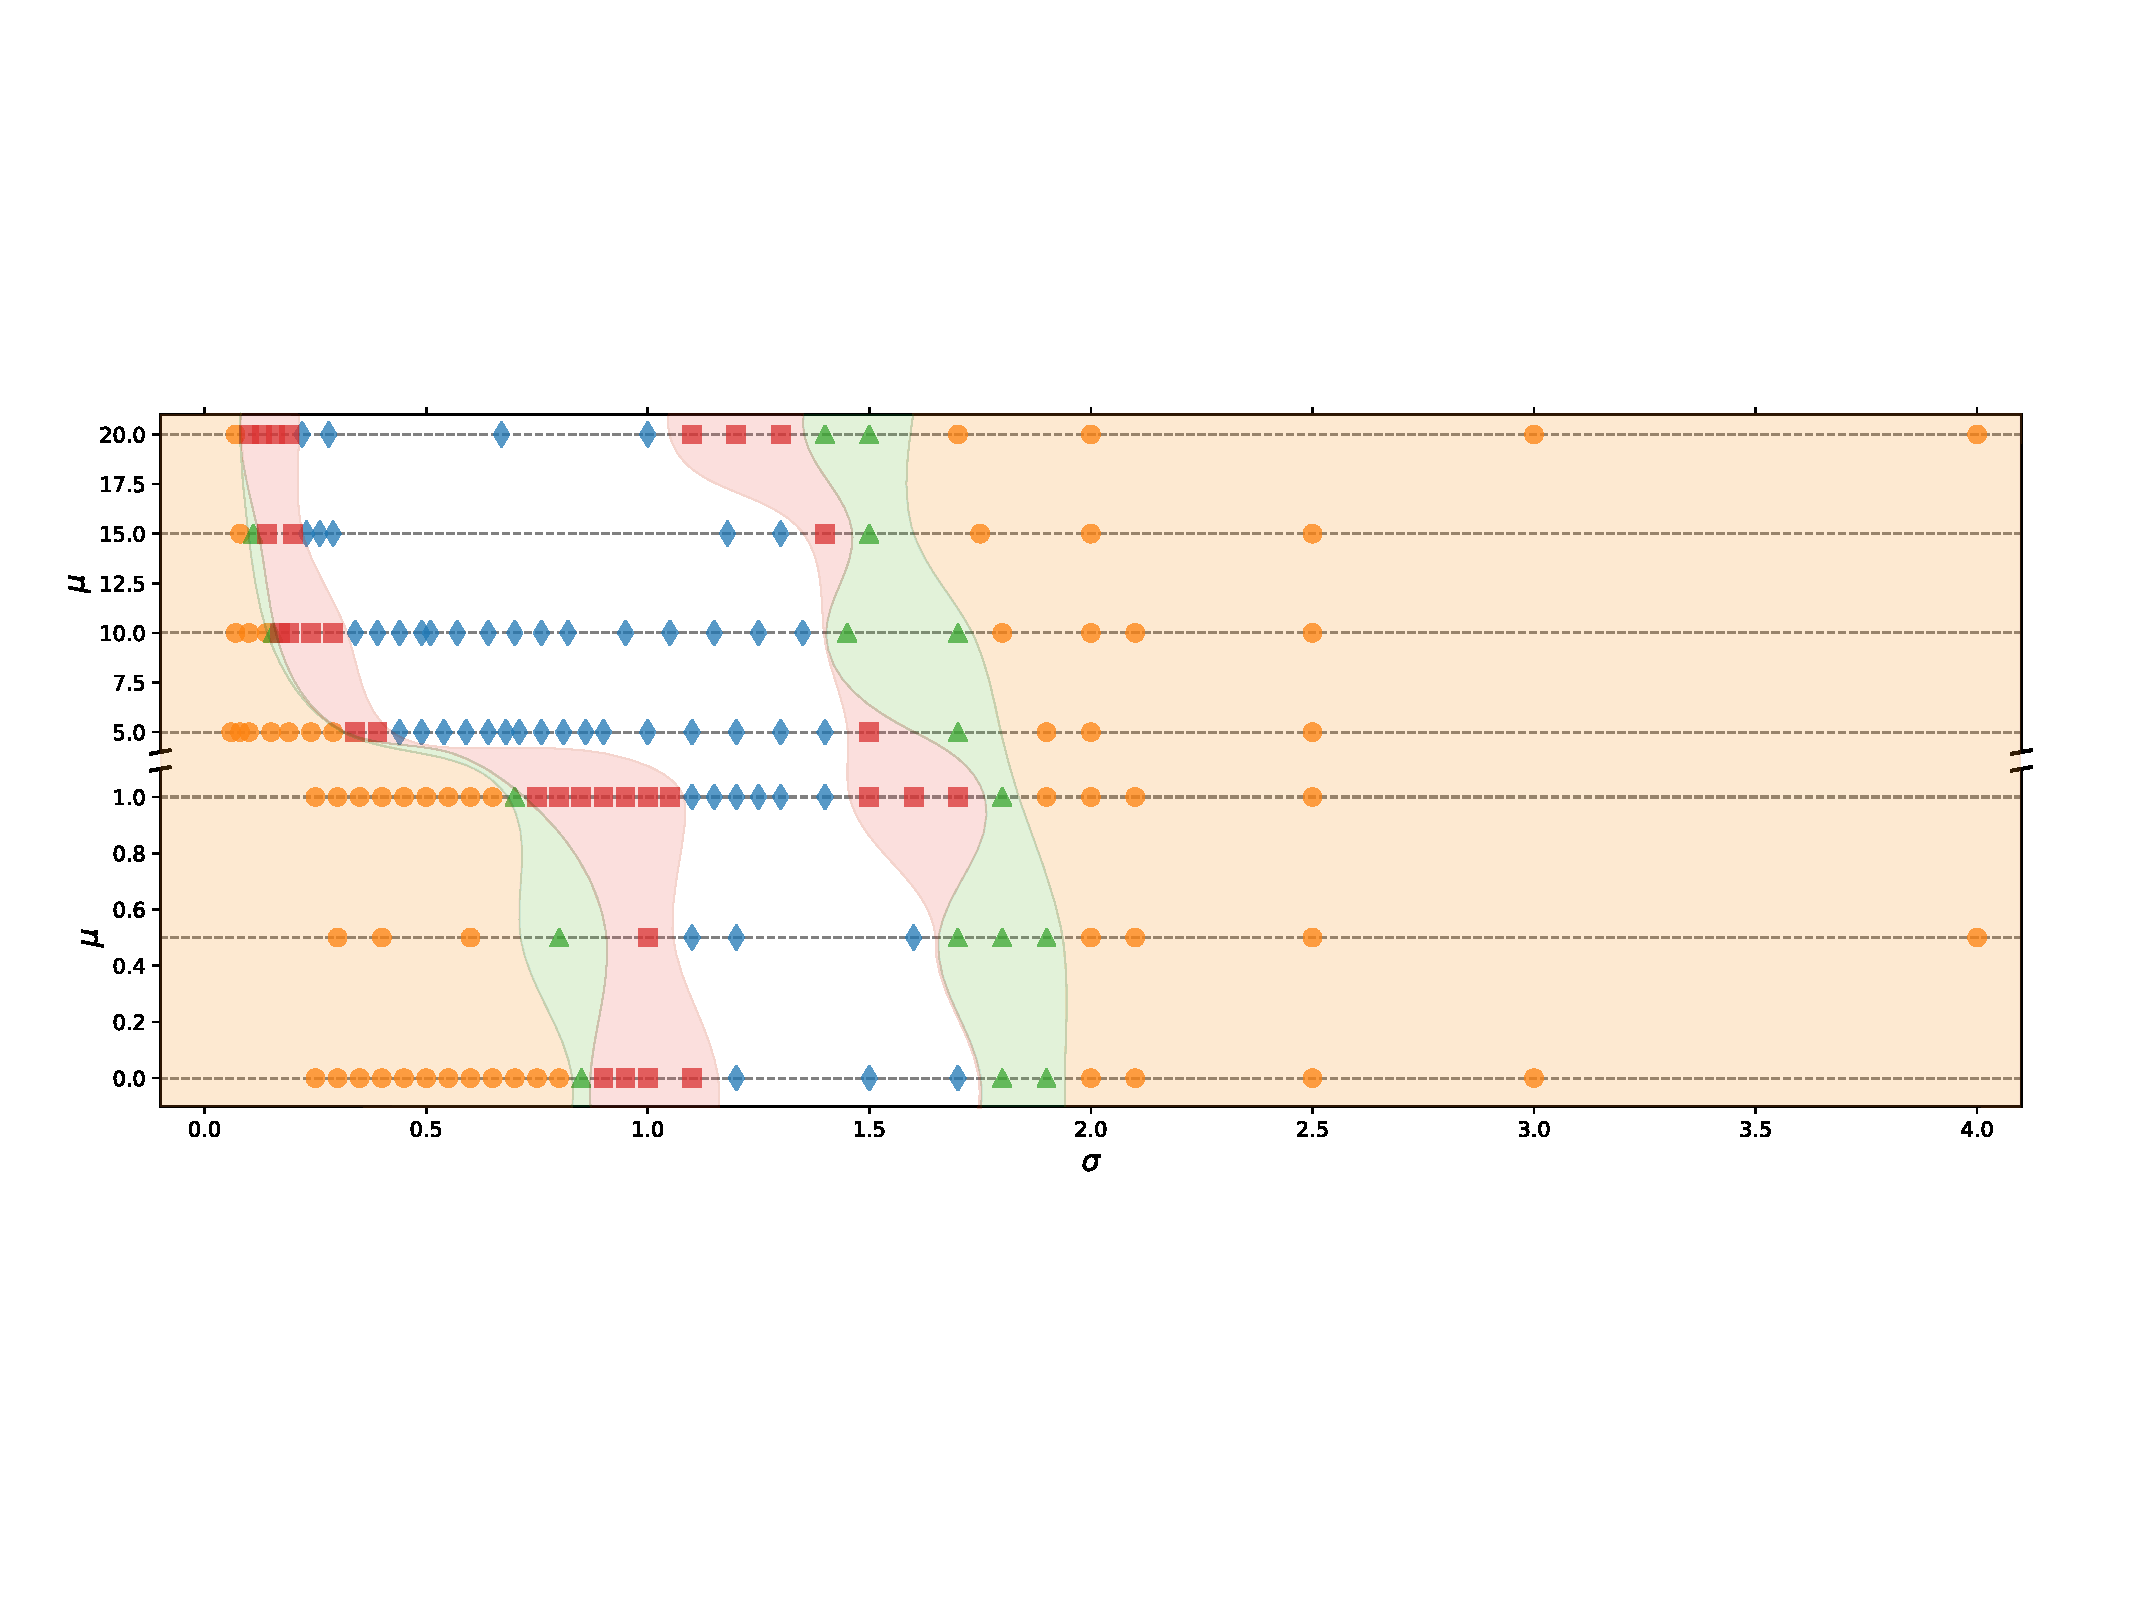
\includegraphics[width=\textwidth]{phase_sections3}
  \end{center}
  }
\only<5>{
  \begin{center}
  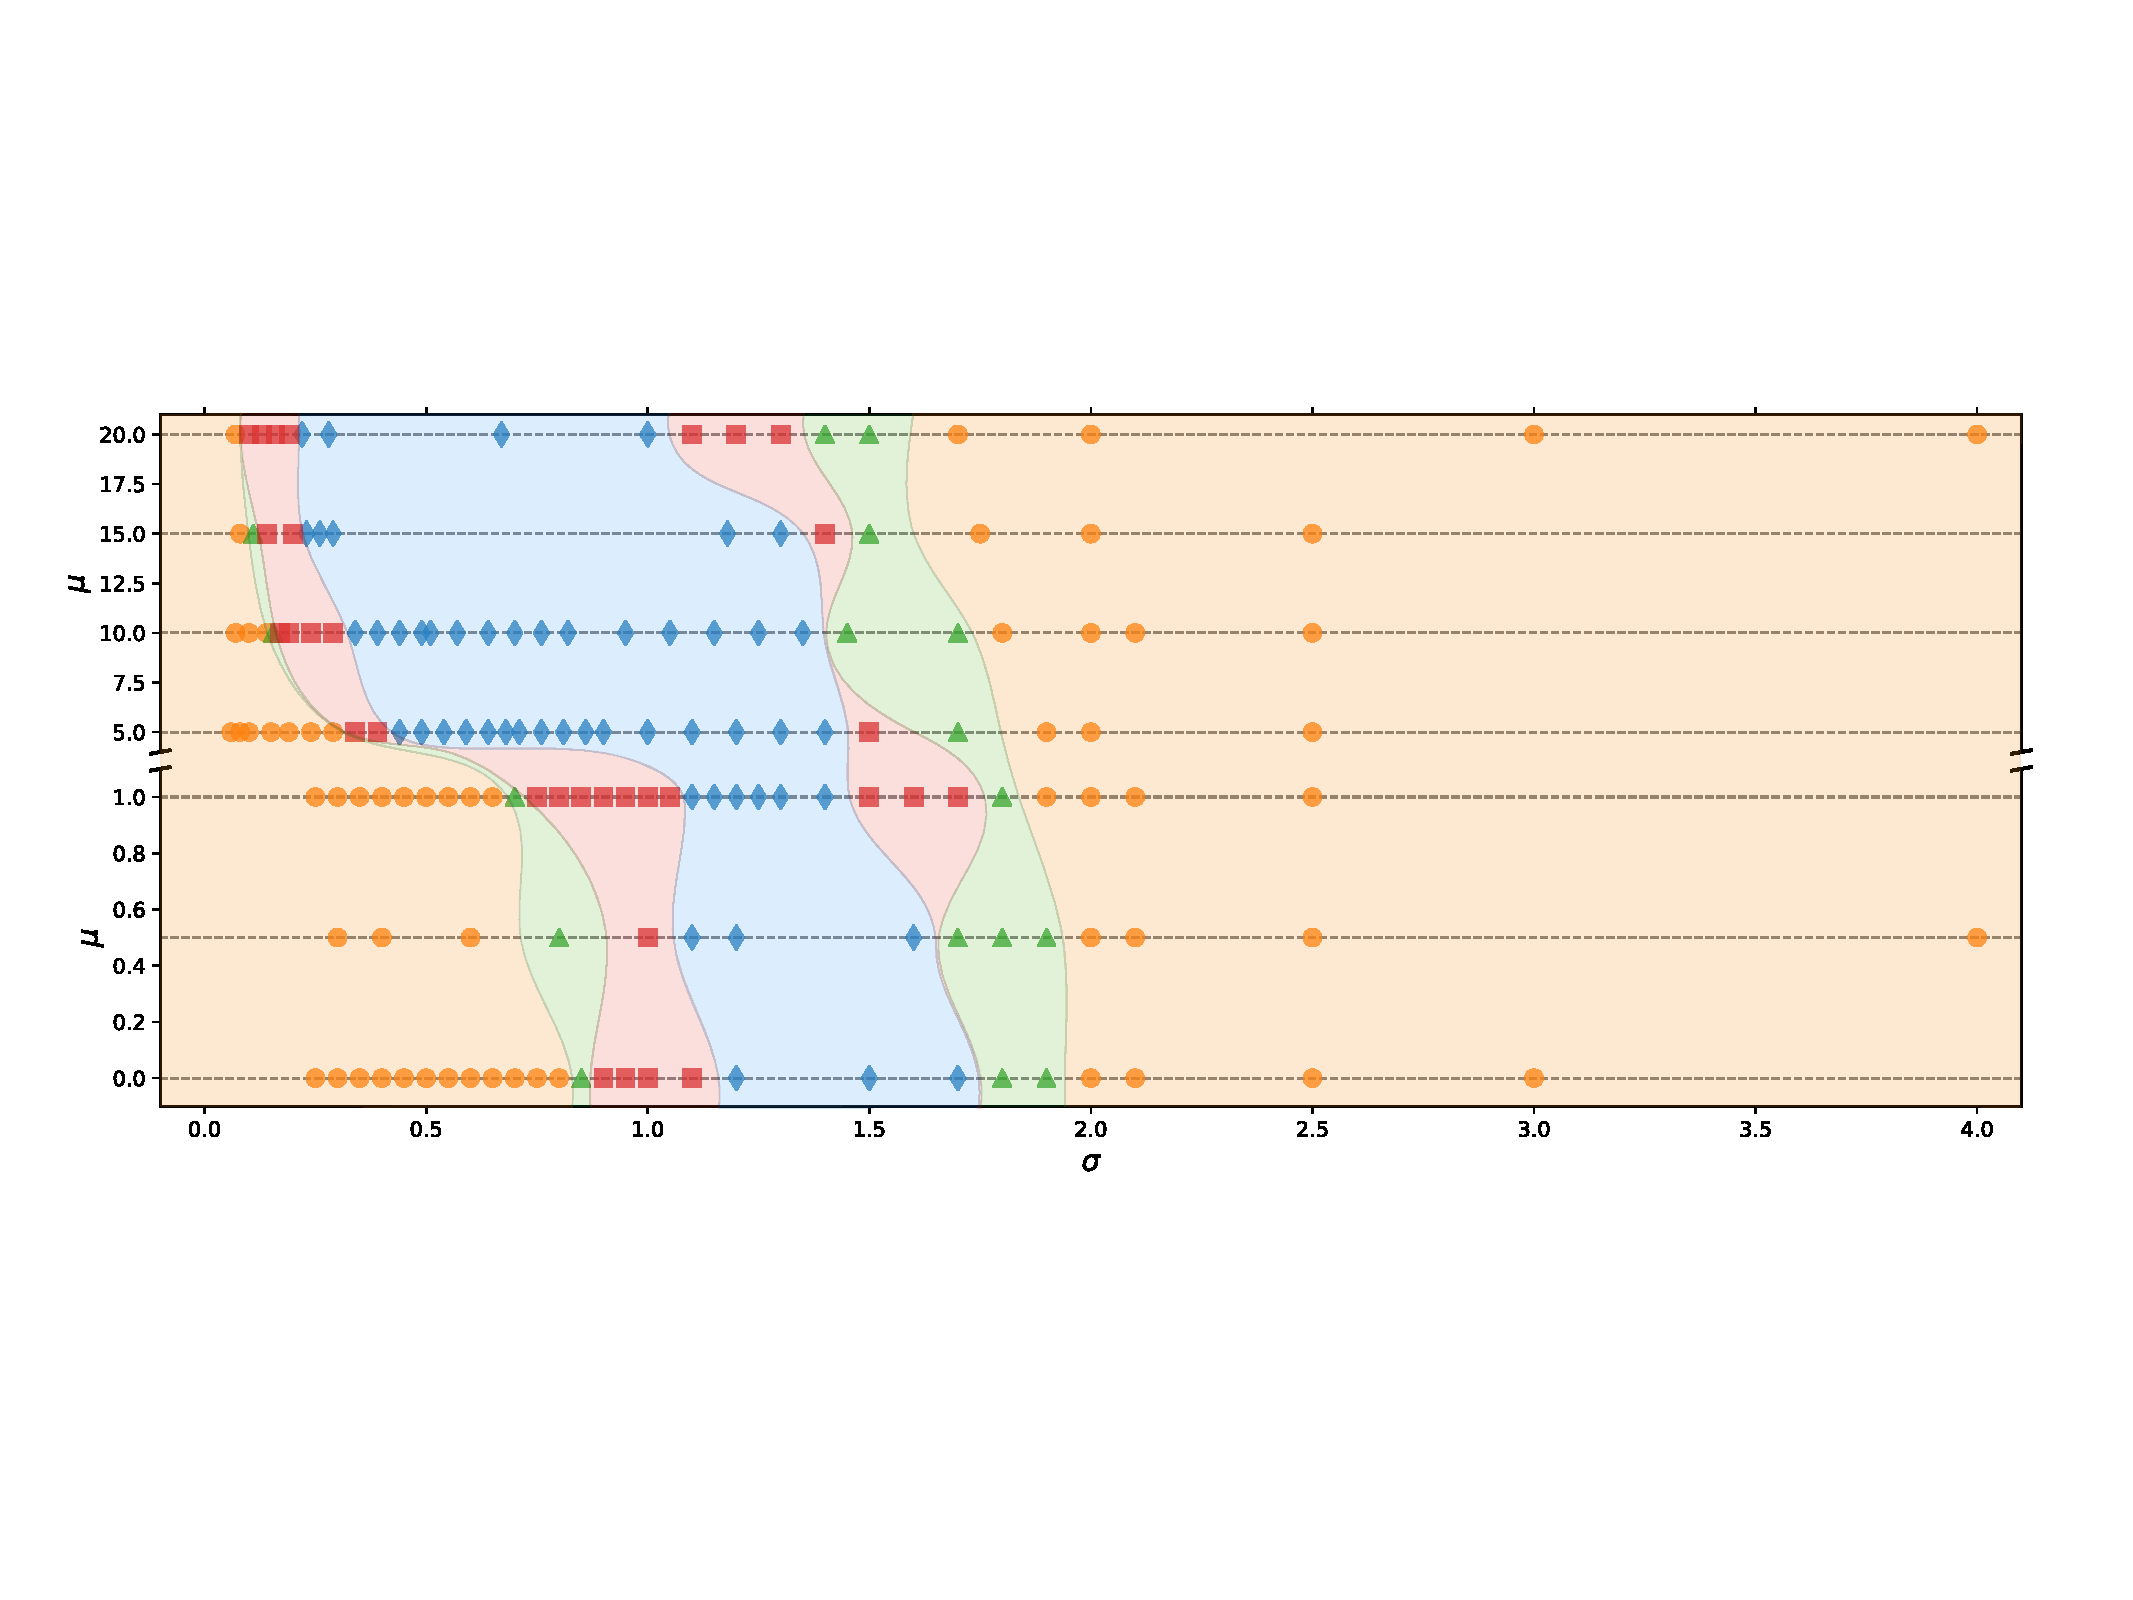
\includegraphics[width=\textwidth]{phase_sections4}
  \end{center}
  }
  \end{figure}
}

\frame
{
  \frametitle{Energy Cascades}
  \bi
  \its Stable solutions: \alert{direct} and \alert{inverse} energy cascades
  \ei
  \begin{columns}
  \column{0.5\textwidth}
      \begin{figure}
      \centering
      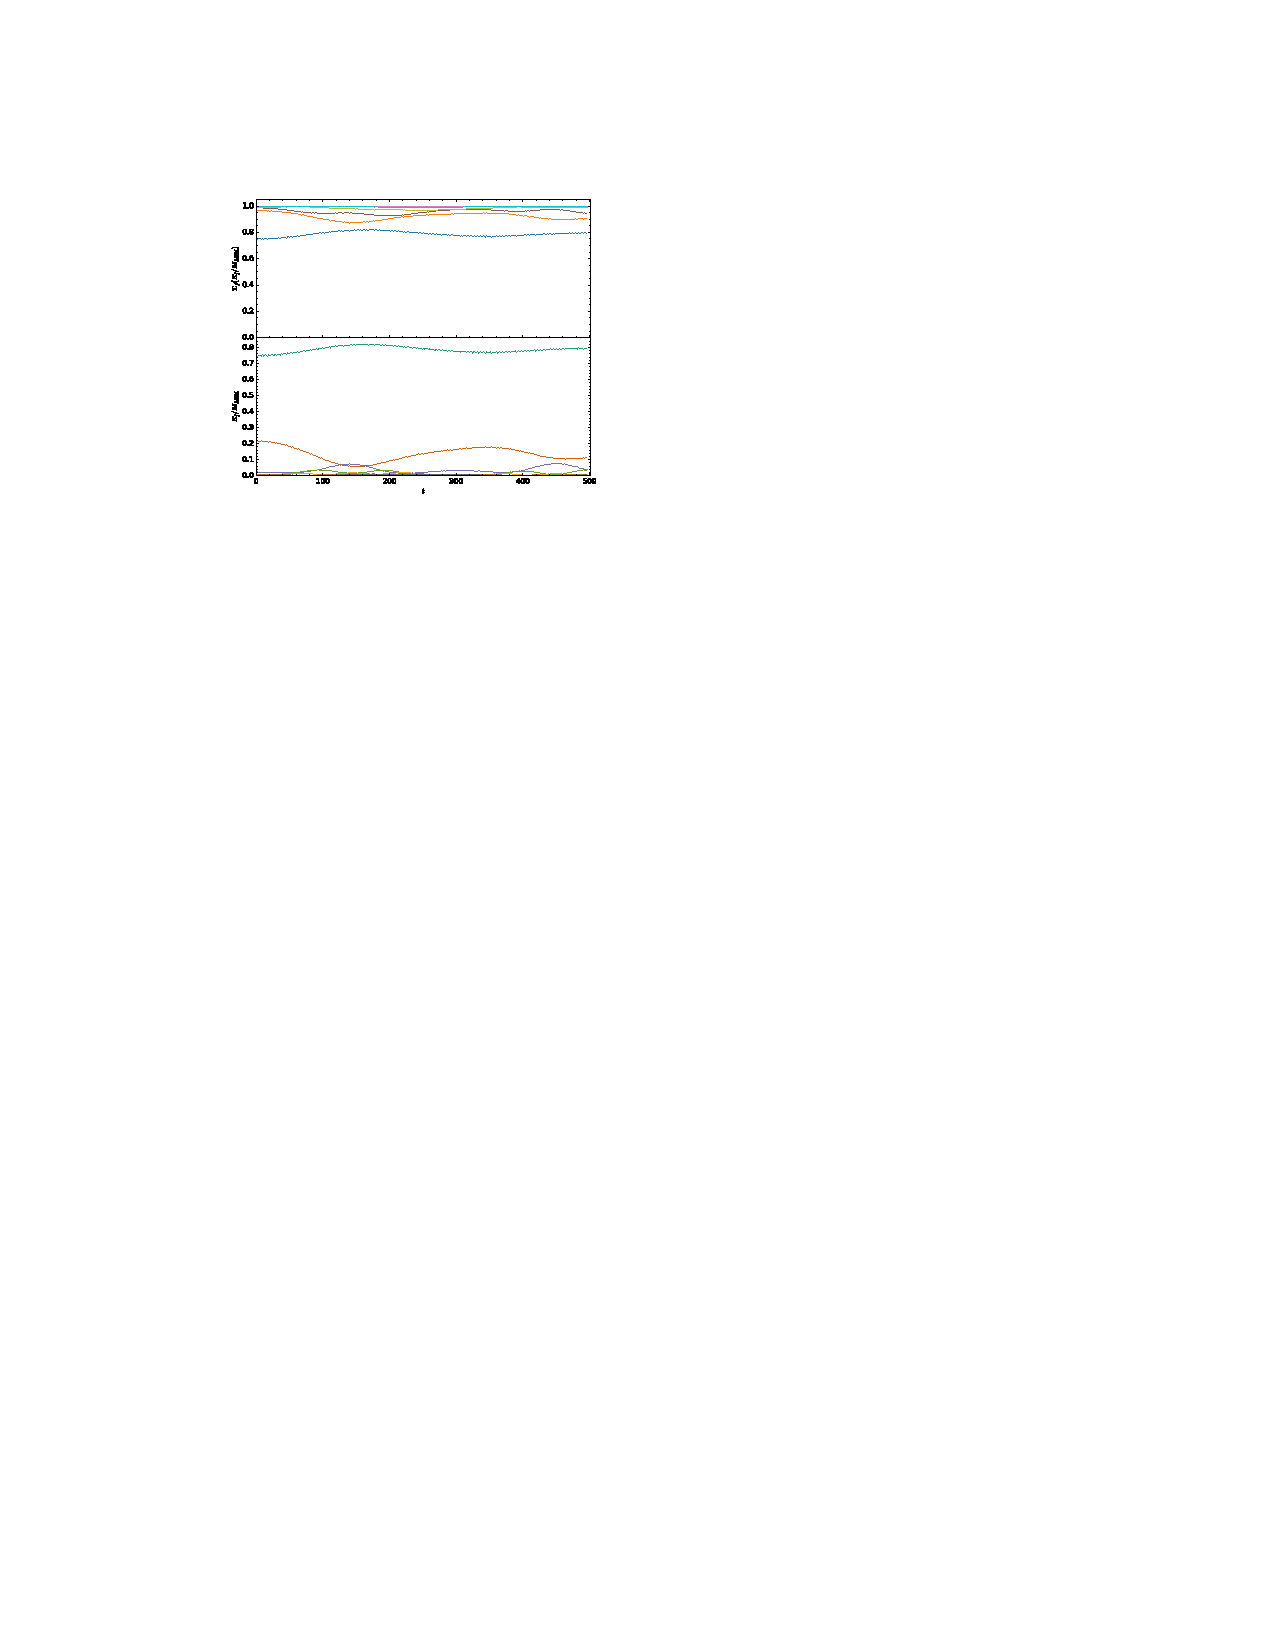
\includegraphics[width=\textwidth]{Em0w18} \\ $\mu = 0$, $\sigma = 1.8$, $\epsilon=0.13$ \\ Stable
      \end{figure}
  \column{0.5\textwidth}
      \begin{figure}
      \centering
      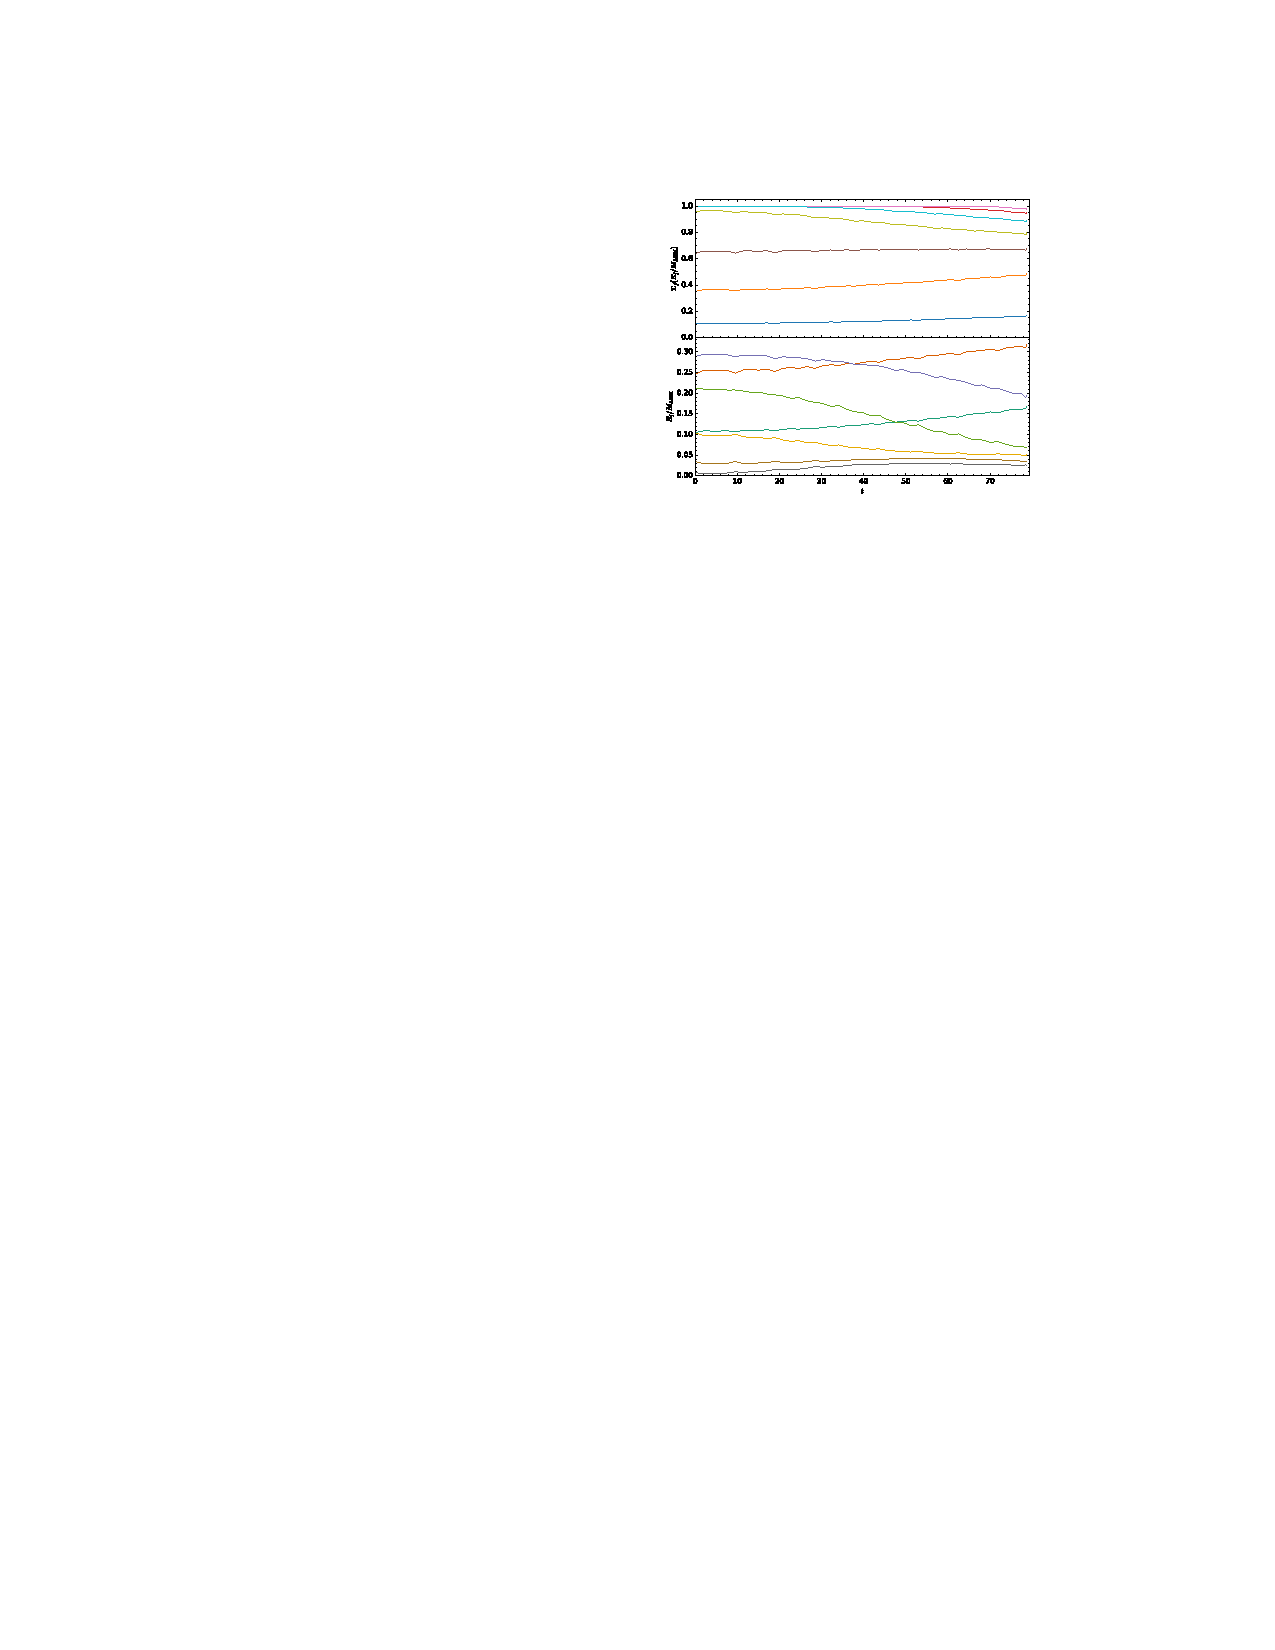
\includegraphics[width=\textwidth]{Em0w025} \\ $\mu = 0$, $\sigma = 0.25$, $\epsilon=2.28$ \\ Unstable
      \end{figure}
  \end{columns}
}

\subsection*{}  
\frame
{
  \frametitle{Results}
  \bi
  \its First full phase diagram of stability in AdS$_5$ $\to$ islands of stability and ``shorelines''
  \its Evidence of metastable and irregular phases at finite $\epsilon$
  \its Fate of metastable phase as $\epsilon \to 0$ yet to be determined
  \its Irregular phase contains quasi-stable initial data\footnotemark$^{,}$\footnotemark $\to$ first evidence for weakly chaotic evolution in massless, spherically-symmetry scalars in AdS
  \its Metastable and irregular data to be studied in multiscale perturbation theory
  \ei
  
  \footnotetext[6]{{\scr Deppe \& Frey [1508.02709]}}
  \footnotetext[7]{{\scr Buchel {\it et al.} [1304.4166]}}
}  
  
%%%%%%%%%%%%%%%%%%%%%%%%%%%%%%%%%%%%%%%%%%%%%%
%%%%%%%%%%%%%%%%%%%%%%%%%%%%%%%%%%%%%%%%%%%%%%

\section{High-Temperature QP Solutions in AdS$_4$}

\subsection{The Two-Time Formalism (TTF)}
\frame
{
  \frametitle{The Two-Time Formalism (TTF) I}
  \vspace{-0.75in}
  \bi
  \its Small perturbations in AdS$_4$: expand scalar field, metric functions in $\epsilon$
  \its $\mc O(\epsilon)$: $\phi_1$ in terms of eigenfunctions of AdS, \alert<1>{$e_j(x)$}
  \its Integer eigenvalues $\omega_j = (2j + d)$ $\to$ fully resonant spectrum
  \its $\mc O(\epsilon^2)$: backreaction on metric in terms of $\phi_1$
  \its <2->{$\mc O(\epsilon^3)$: \alert{source terms} for resonant contributions }
  \its<2->{Define slow time $\tau \equiv \epsilon^2 t$}
  \ei

  \begin{overlayarea}{\textwidth}{0.1cm}
  \begin{align*}
  \only<1>{
  \vspace{0.4in}
  \phi_1 (t,x) = \sum^\infty_{j=0} A_j(t) \cos (\omega_j t + B_j(t)) \: \alert{e_j (x)}
  }
  \only<2>{
  \vspace{-0.3in}
   -\! 2 \omega_\ell \frac{d A_\ell (\tau)}{d \tau} &= \stackrel{\ell \leq i + j}{\sum_{i \neq \ell} \sum_{j \neq \ell}} \alert{f_1} \left(A_i, A_j, A_{i+j-\ell}, B_i, B_j, B_{i+j-\ell} \right) \\
  -2 \omega_\ell A_\ell \frac{d B_\ell(\tau)}{d \tau} &= \stackrel{\ell \leq i + j}{\sum_{i \neq \ell} \sum_{j \neq \ell}} \alert{f_2} \left(A_i, A_j, A_{i+j-\ell}, B_i, B_j, B_{i+j-\ell} \right)
  }
  \end{align*}
  \end{overlayarea}
  \vspace{0.41in}
}

\frame
{
  \frametitle{The Two-Time Formalism (TTF) II}
  \bi
  \its Energy exchange between modes through slowly varying amplitude $A_j(\tau)$ and phase $B_j(\tau)$ to resist collapse\footnotemark
  \its Resummation techniques absorb resonances into amplitude/phase variables\footnotemark
  \its Solve by truncating series to $\jm < \infty$
  \its Solutions must be robust as $\jm \to \infty$
  \its Examine quasi-periodic families of solutions\footnotemark
  \its Develop numerical techniques for extending $\jm \gtrsim 100$
  \its Verify families of solutions remain valid as $\jm$ increases
  \ei
  
  \footnotetext[8]{{\scr Balasubramanian {\it et al.} [1403.6471]}}
  \footnotetext[9]{{\scr Craps {\it et al.} [1407.6273]}}
  \footnotetext[10]{{\scr Green {\it et al.} [1507.08261]}}
}

%%%%%%%%%%%%%%%%%%%%%%%%%%%%%%%%%%%%%%%%%%%%%%

\subsection{Quasi-Periodic Solutions}
\frame
{
  \frametitle{Quasi-Periodic Solutions I}
  \bi
  \its Quasi-periodic ansatz $A_j = \alpha_j e^{i \beta_j \tau}$ $\to$ TTF equations become time-independent when $\beta_j = \beta_0 + j(\beta_1 - \beta_0)$
  \its Solve QP equation with Newton-Raphson $\to$ seed equation $\alpha_j \propto e^{-j}$, $j \neq 0$ for low $\jm$
  \its TTF: conserved quantities\footnotemark\ $E$, $N$ $\to$ classify solutions by $T \equiv E/N$
  \its $T_i$, $R_{ij}$, $S_{ijk\ell}$ calculated numerically
  \ei
  
   \begin{align*}
  2\omega_\ell \alpha_\ell \beta_\ell = T_\ell \alpha_\ell^3 + \sum_{i \neq \ell} R_{i\ell} \alpha_i^2 \alpha_\ell + \stackrel{\ell \leq i + j}{\sum_{i \neq \ell} \sum_{j \neq \ell}} S_{i j (i+j-\ell)\ell} \alpha_i \alpha_j \alpha_{i+j-\ell}
  \end{align*}
 
 \footnotetext[11]{{\scr Craps {\it et al.} [1412.3249]}}
}

\frame
{
  \frametitle{Quasi-Periodic Solutions II}
  \bi
  \its Solutions found for $3 \geq T \gtrsim 4.6$
  \its Able to extend existing solutions from $\jm \sim 100$ to $\jm = 500$
  \its Robust in $\jm \to \infty$ limit
  \ei
  
  \vspace{-0.1in}
  \begin{columns}
  \column{0.5\textwidth}
  \begin{figure}
  \centering
  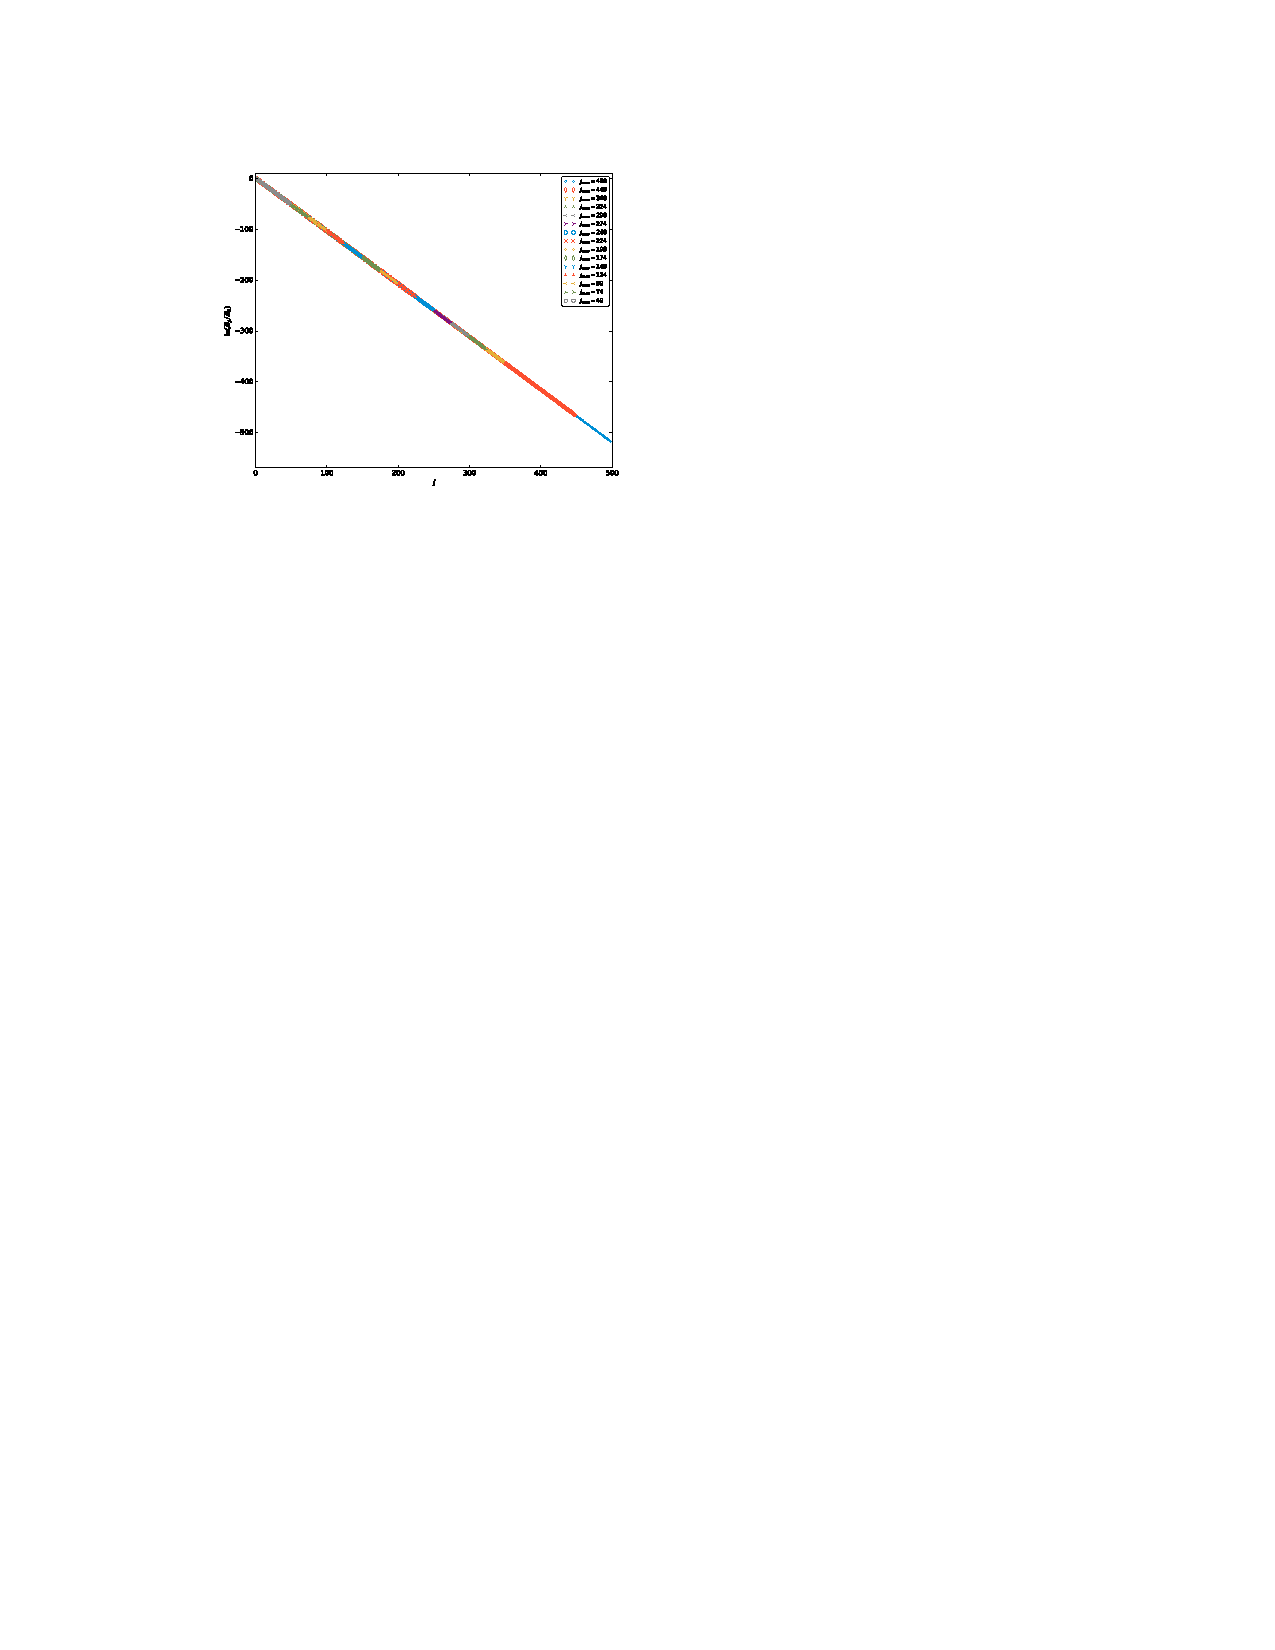
\includegraphics[scale=0.75]{largejmax} 
  \end{figure}
  \column{0.5\textwidth}
  \begin{figure}
  \centering
  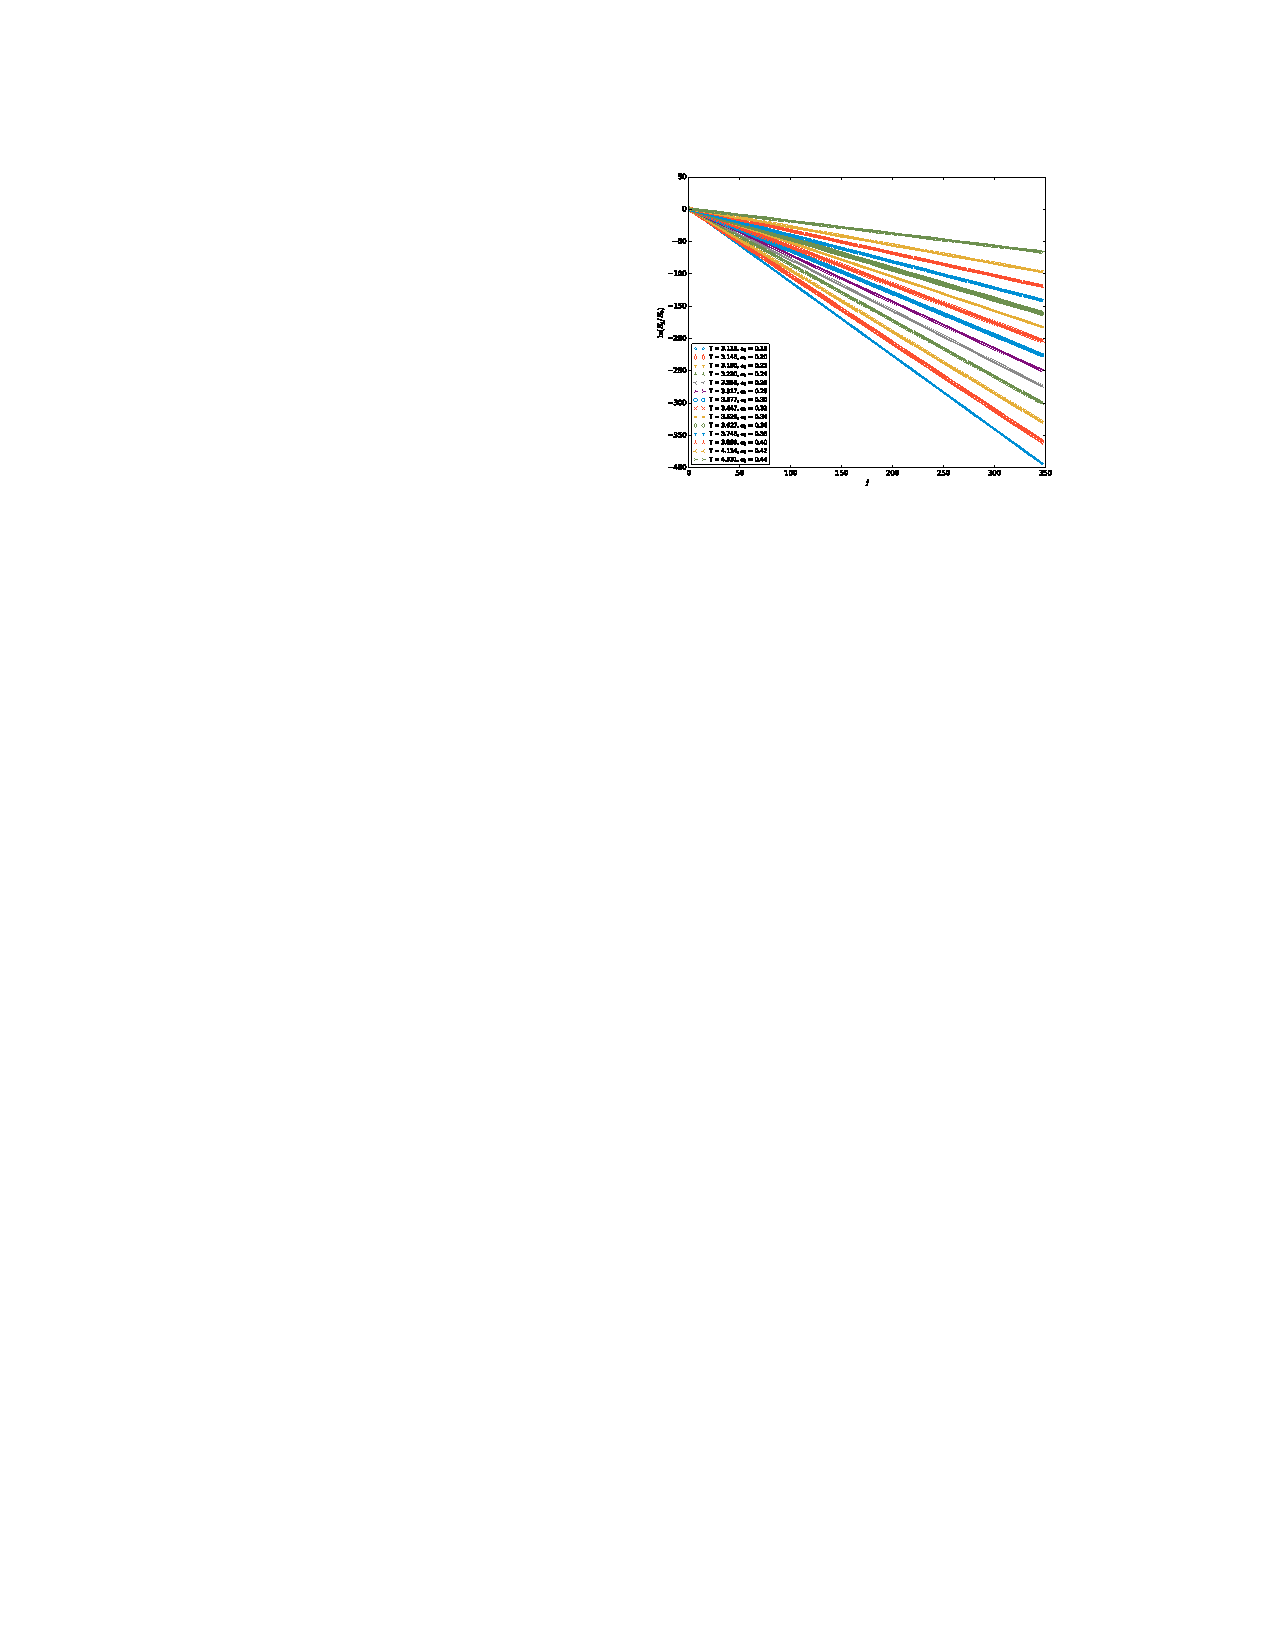
\includegraphics[scale=0.75]{families}
  \end{figure}
  \end{columns}
  \begin{center}
  {\scr BC, Deppe, \& Frey: In progress}
  \end{center}
  
  \vfill
}

%%%%%%%%%%%%%%%%%%%%%%%%%%%%%%%%%%%%%%%%%%%%%%

\subsection{High-Temperature Families}
\frame
{
  \frametitle{High-Temperature Solutions I}
  \bi
  \its Perturb by $\delta E$ $\to$ new solutions have energy $E + \delta E$, $N$, and $T + \delta T$
  \its Repeat process to $T_{max} = (2\jm + d)$
  \its Project back to QP solution surface at constant $\alpha_1$ or $T$
  \its Loss of smooth profile above a certain temperature at \alert<1>{constant $\alpha_1$} 
  \ei
  
  \vspace{-0.15in}
  \begin{columns}
  \column{0.5\textwidth}
  \begin{figure}
  \centering
  \hspace{0.1in}
  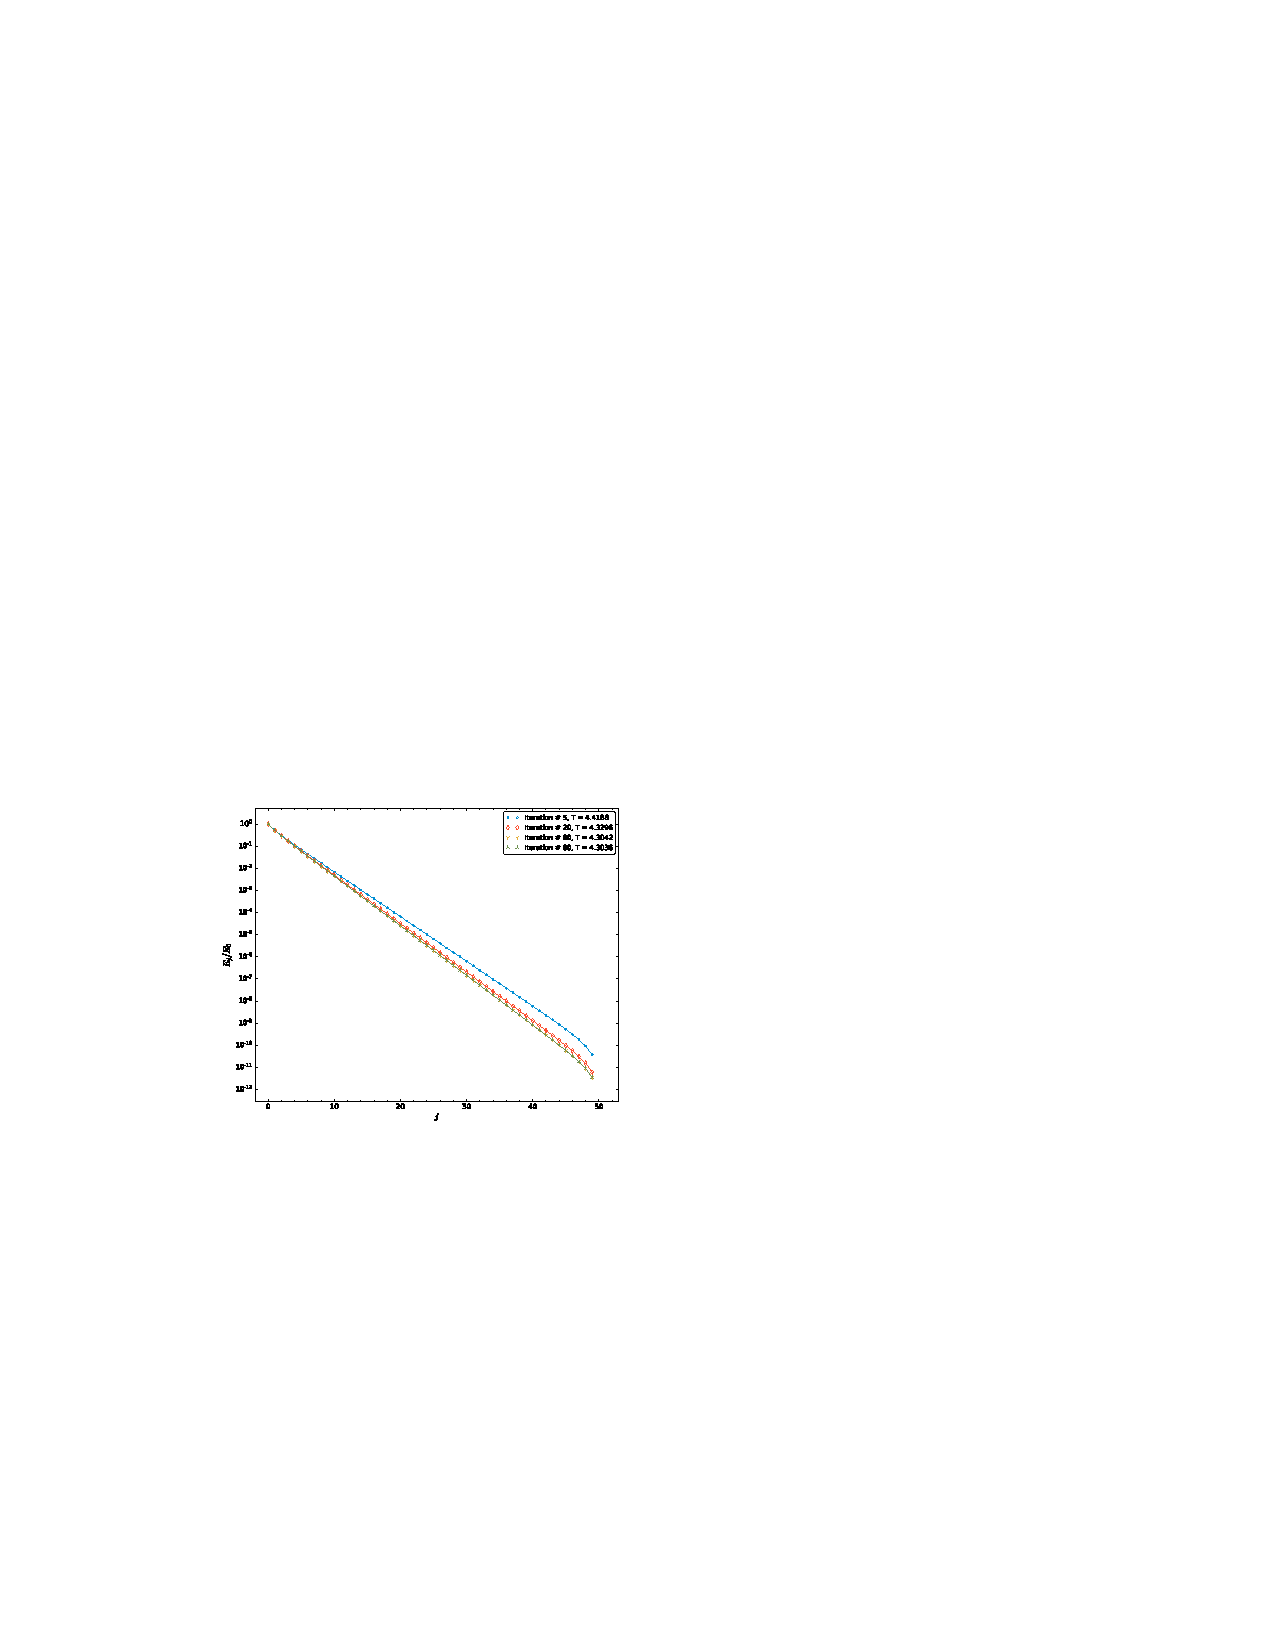
\includegraphics[scale=0.75]{reop5}
  \end{figure}
  \column{0.5\textwidth}
  \begin{figure}
  \centering
  \hspace{-0.1in}
  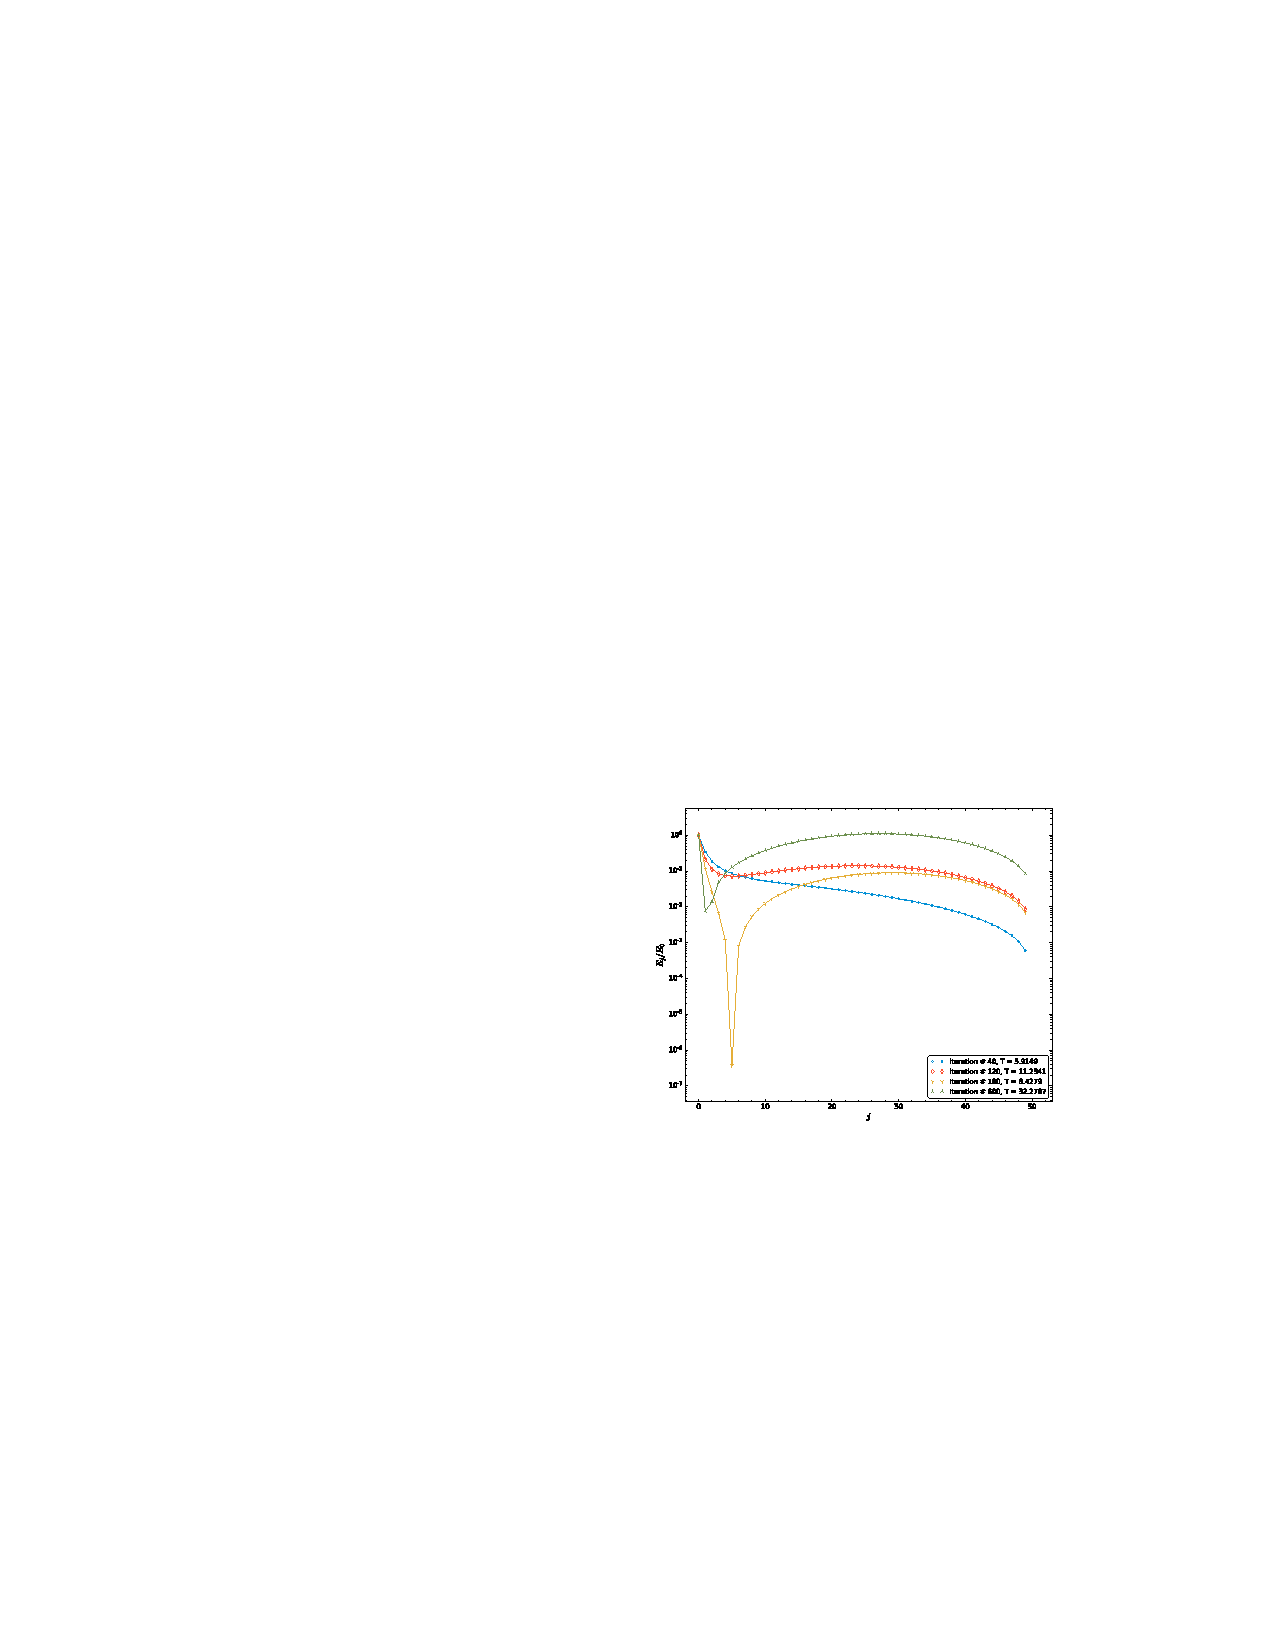
\includegraphics[scale=0.75]{reop20}
  \end{figure}
  \end{columns}
  \begin{center}
  \vspace{-0.12in}
  {\scr Cownden, Deppe, \& Frey: In progress}
  \end{center}
  \vspace{-0.1in}
%\marginnote{\pdfcomment[icon=note]{(L) reop 5}}
%\marginnote{\pdfcomment[icon=note]{(R) reop 20}}
}

\frame
{
  \frametitle{High-Temperature Solutions II}
  \bi
  \its And at \alert{constant T}
  \ei
   \begin{figure}
    \centering
    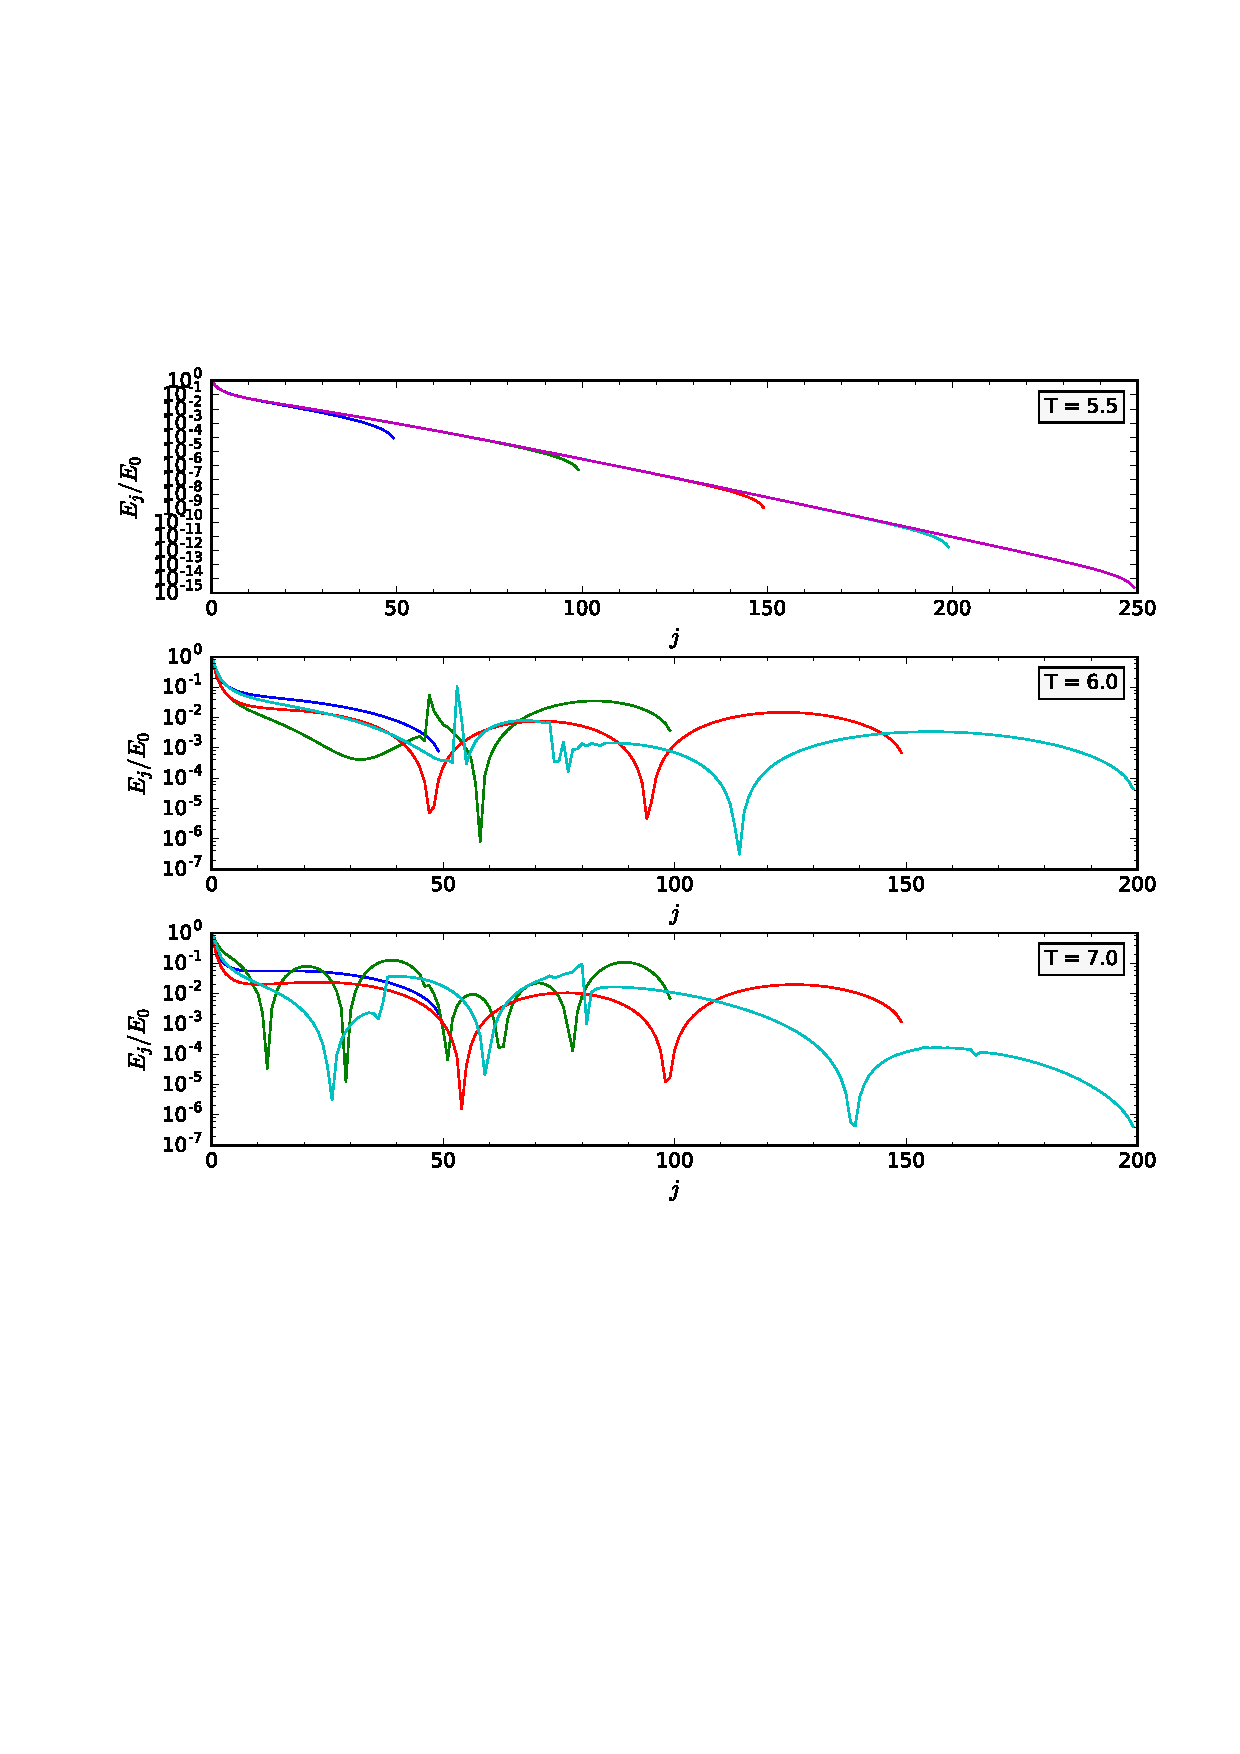
\includegraphics[scale=0.43]{constantTproj} \\ {\scr Cownden, Deppe, \& Frey: In progress}
  \end{figure}
}

\frame
{
  \frametitle{High-Temperature Solutions III}
  \bi
  \its Alternative methods for finding high-T solutions
  \its<2->{Fit low $\jm$, high-T data to generate seeds for Newton-Raphson solver \uncover<3->{$\to$ \alert<3>{not robust as $\jm$ increases}}}
  \its<4->{Pad low $\jm$ data with zeros, evolve within the TTF \uncover<5->{$\to$ \alert<5>{isothermal evolution does not match known solution}}}
   \ei
   \begin{overlayarea}{\textwidth}{0.65\textheight}
      \begin{figure}
      \centering
      \only<2-3>{
      \vspace{-0.35in}
      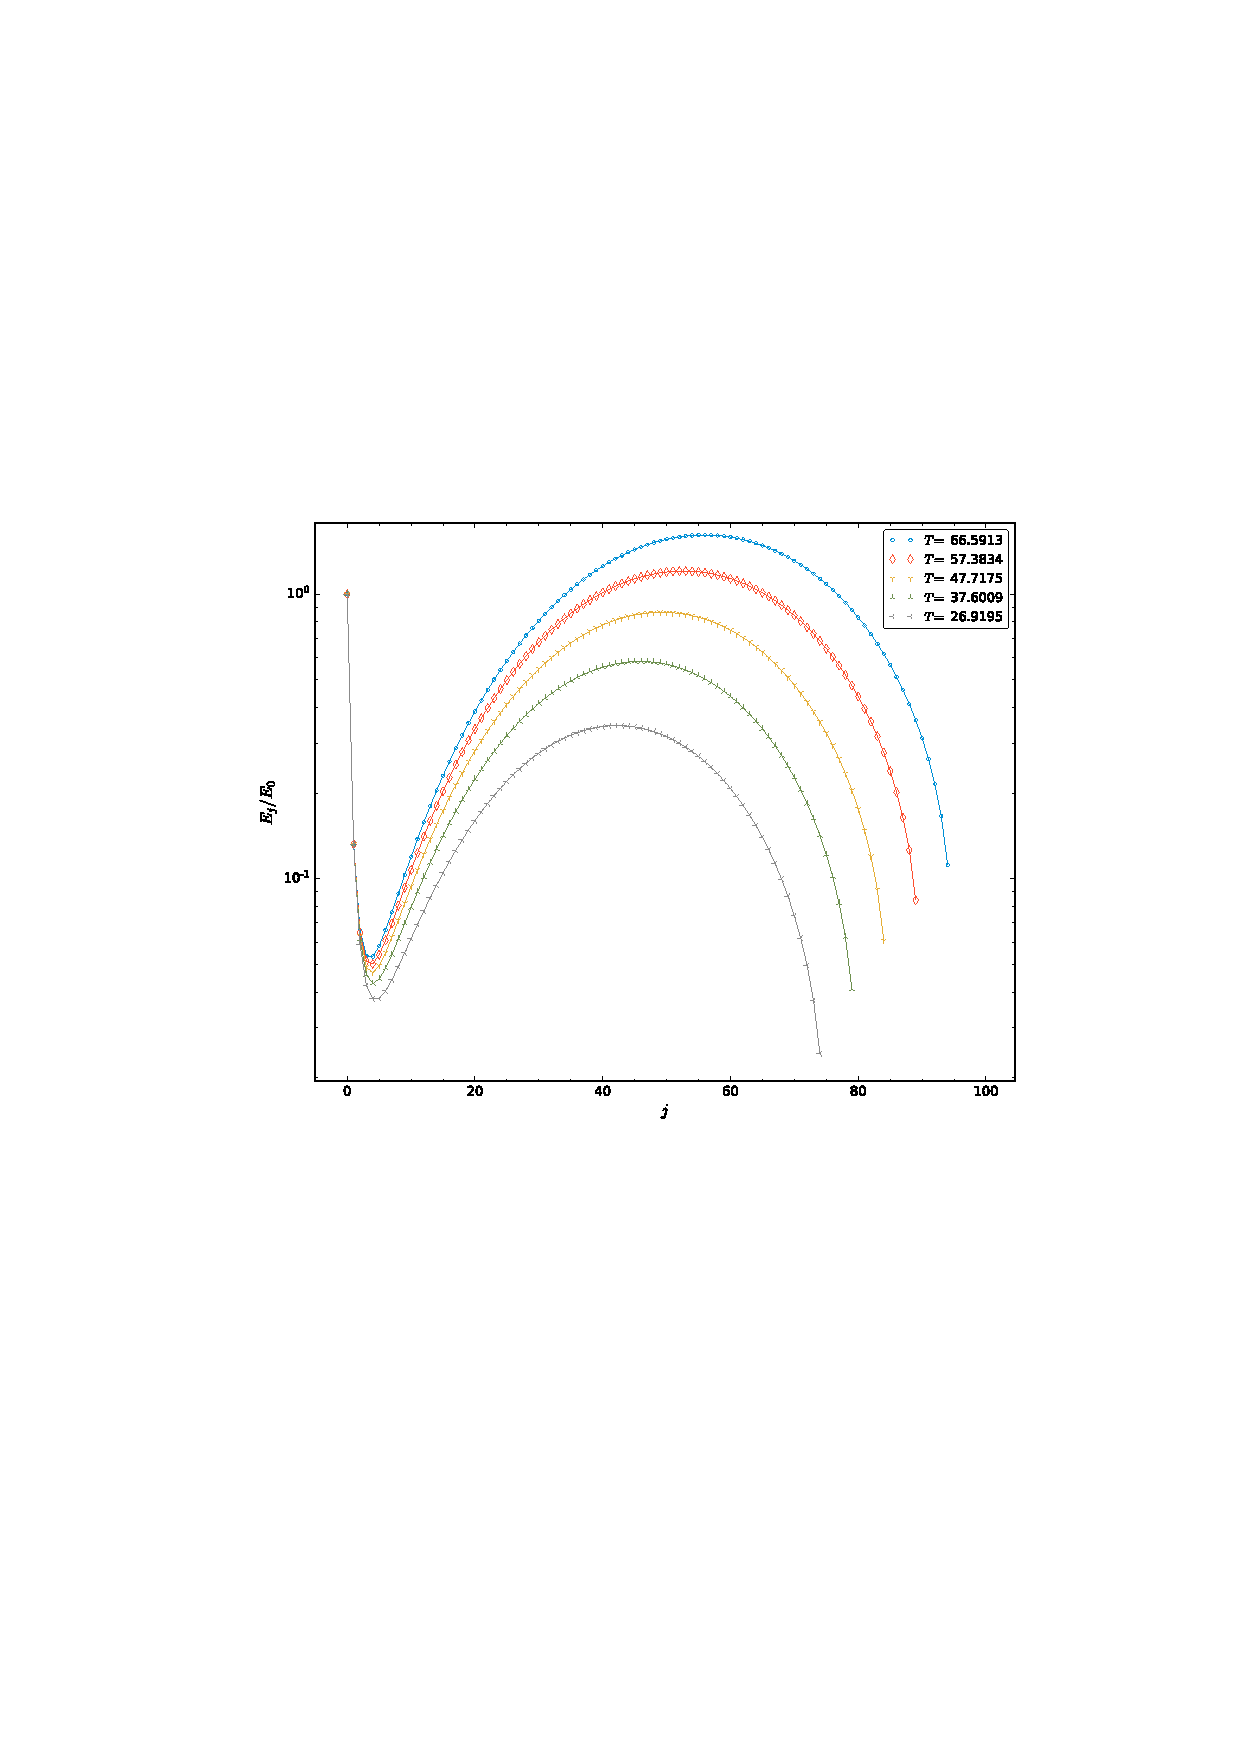
\includegraphics[scale=0.6]{highTseeds}
      }
      \only<4->{
      \includegraphics[scale=1.0]{TTFEvo}
      }
      \end{figure}
  \end{overlayarea}
}

\subsection*{}
\frame
{
  \frametitle{Results}
    \bi
    \its Low-T QP solutions robust as $\jm$ increases
    \its Not able to find evidence that high-T solutions continued to exist at large $\jm$ $\to$ possible reduction of space of QP solutions up to $T_{max} = 2\jm + d$
    \its {\bf Caveat}: focused on configurations where $\alpha_0 = 1$ $\to$ free to set dominant energy in any $\alpha_j$
    \its Motivation for temperature limit of $T \sim 5.5$?
    \its Perturbative system: massless scalar, static boundary conditions at $x = \pi/2$
    \its Extend to massive scalars, time-dependent boundary conditions $\to$ activation of non-normalizable modes
    \ei
}

%%%%%%%%%%%%%%%%%%%%%%%%%%%%%%%%%%%%%%%%%%%%%%
%%%%%%%%%%%%%%%%%%%%%%%%%%%%%%%%%%%%%%%%%%%%%%

\section{Examining Instabilities Due to Driven Scalars in AdS [arXiv:1912.07143]}
\subsection{Extending TTF to Driven Scalars}
\frame
{
  \frametitle{Extending TTF to Driven Scalars}
  \bi
  \its Driven scalars $\to$ scalars with time-dependent boundary conditions at $x = \pi / 2$
  \its $\mc O(\epsilon)$: $\phi_1(t, x=\pi/2) = f(t)$
  \its<2->{Examine scaling behaviour as $x \to \pi/2$: $\Phi^+(x) \sim (\cos x)^{\Delta^+}$ and $\Phi^-(x) \sim (\cos x)^{\Delta^-}$}
  \its<3->{Scalar field is linear combination of both kinds of modes}
  \its<3->{\alert<3>{$e_j(x)$} are same eigenfunctions of AdS \& have eigenvalues \alert<3>{$\omega_j = (2j + \Delta^+)$}}
  \its<4->{\alert{$E_\alpha(x)$} are hypergeometric functions \& have continuous eigenvalues \alert{$\omega_\alpha$}}
  \ei
  \vspace{-0.2in}
  \begin{overlayarea}{\textwidth}{0.25\textheight}
  \begin{align*}
  \only<2>{
    \Phi^+(x) \equiv \text{``normalizable''} \quad & \quad \Phi^-(x) \equiv \text{``non-normalizable''}
    }
  \only<3->{
    \phi_1(t,x) = \sum_{j=0}^\infty A_j(t) \cos & \left(\alert<3>{\omega_j} t + B_j (t)\right) \alert<3>{e_j(x)} + \sum_{\alpha = 0}^\infty \bar{A}_\alpha(t) \cos \left( \alert<4>{\omega_\alpha} t + \bar{B}_\alpha \right) \alert<4>{E_\alpha (x)} \\
    & \alert<3>{\Delta^\pm = \frac{d}{2} \pm \frac{1}{2} \sqrt{d^2 - 4m^2}}
    }
  \end{align*}
  \end{overlayarea}
  \vspace{0.3in}
}

%%%%%%%%%%%%%%%%%%%%%%%%%%%%%%%%%%%%%%%%%%%%%%

\subsection{Resonant Contributions}
\frame
{
  \frametitle{Resonant Contributions}
  \bi
  \its $\mc O(\epsilon^2)$: backreaction on metric in terms of $\phi_1$
  \its $\mc O(\epsilon^3)$: source terms for resonant contributions $\to$ examine resonance conditions 
  \its<2->{\alert<2>{All normalizable}: restrictions on indices {\bf and} mass value}
  \ei
  
  \begin{overlayarea}{\textwidth}{0.25\textheight}
  \begin{align*}
  \only<2>{
  \omega_i + \omega_j + \omega_k &= \omega_\ell \quad \Rightarrow \quad i + j + k = \ell - \Delta^+  \in \mathbb{Z}^+ \\
  \omega_i - \omega_j - \omega_k &= \omega_\ell \quad \Rightarrow \quad i - j - k = \ell + \Delta^+  \in \mathbb{Z}^+ \\
  \omega_i + \omega_j - \omega_k &= \omega_\ell \quad \Rightarrow \quad i + j = k + \ell \, \in \mathbb{Z}^+
  }
  \end{align*}
  \end{overlayarea}
}

%%%%%%%%%%%%%%%%%%%%%%%%%%%%%%%%%%%%%%%%%%%%%%

\subsection{Special Values of Non-normalizable Frequencies}
\frame
{
  \frametitle{Special Values of Non-normalizable Frequencies}
}

%%%%%%%%%%%%%%%%%%%%%%%%%%%%%%%%%%%%%%%%%%%%%%
%%%%%%%%%%%%%%%%%%%%%%%%%%%%%%%%%%%%%%%%%%%%%%

{
  \AtBeginSection[]{}
\section{Conclusions}
\frame
{
   \frametitle{Conclusions}
   \bi
   \its Collapse of scalar field in AdS $\Leftrightarrow$ thermalization of dual CFT
   \its {\bf Nonlinear theory:} ``islands of stability'', metastable \& irregular phases, chaotic behaviour from self-interaction
   \its Weakly turbulent energy cascade to short length scales $\to$ TTF for inverse cascades 
   \its {\bf Perturbative theory:} QP solutions robust in $j_{max} \to \infty$, high-T solutions are not; space of stable solutions is restricted by $T_{th}$
   \its {\bf Next steps}
     \begin{itemize}
     \its Physical interpretation of $T_{th}$ 
     \its Ways to construct robust QP solutions with $T > T_{th}$
     \end{itemize}
   \its {\bf Future:} develop theory for \underline{\emph{massive}} TTF $\to$ less symmetry in equations $\therefore$ fewer cancelations of resonant terms; TTF in AdS$_5$; time-dependent boundary conditions
    \ei
}
\section*{}
\frame[noframenumbering]
{
   \frametitle{Thanks}
   \begin{itemize}
   \its Supervisor: Andrew Frey (University of Winnipeg)
   \its PhD Committee: (),  (), (),  ()
   \its Co-authors: Nils Deppe (Cornell), Brayden Yarish (junior collaborator)
   \its University of Winnipeg and University of Manitoba
   \its Westgrid \& Compute Canada
   \end{itemize}
}

\frame[noframenumbering]
{
  \frametitle{References}
  \bi
  \its M. Choptuik, \emph{Universality and scaling in gravitational collapse of a massless scalar field}, Phys. Rev. Lett. 70 (1993) 9-12. 
  \its P. Bizo\'n and A. Rostworowski, \emph{On weakly turbulent instability of anti-de Sitter space}, Phys. Rev. Lett. 107 (2011) 031102, [1104.3702]. 
  \its N. Deppe and A. R. Frey, \emph{Classes of Stable Initial Data for Massless and Massive Scalars in Anti-de Sitter Spacetime}, JHEP 12 (2015) 004, [1508.02709]. 
  \its J. M. Maldacena, \emph{The Large N limit of superconformal field theories and supergravity}, Int. J. Theor. Phys. 38 (1999) 1113, [hep-th/9711200]. 
  \its R. Brito, V. Cardoso, and J. V. Rocha, \emph{Interacting shells in AdS spacetime and chaos}, Phys. Rev. D94 (2016), no. 2 024003, [1602.03535]. 
  \its N. Deppe, A. Kolly, A. R. Frey, and G. Kunstatter, \emph{Black Hole Formation in AdS Einstein-Gauss-Bonnet Gravity}, J. High Energ. Phys. (2016) 2016: 87, [1608.05402].
  \its B. Craps, O. Evnin, and J. Vanhoof, \emph{Renormalization group, secular term resummation and AdS (in)stability}, JHEP 10 (2014) 048, [1407.6273].
   \ei
}

\frame[noframenumbering]
{
  \frametitle{References}
  \bi
  \its A. Buchel, S. L. Liebling, and L. Lehner, \emph{Boson Stars in AdS Spacetime}, Phys. Rev. D87 (2013) 123006, [1304.4166].
  \its V. Balasubramanian, A. Buchel, S. R. Green, L. Lehner, and S. L. Liebling, \emph{Holographic Thermalization, Stability of Anti-de Sitter Space, and the Fermi-Pasta-Ulam Paradox}, Phys. Rev. Lett. 113 (2014) 071601, [1403.6471].
  \its S. R. Green, A. Maillard, L. Lehner, and S. L. Liebling, \emph{Islands of stability and recurrence times in AdS}, Phys. Rev. D92 (2015) 084001, [1507.08261].
  \its B. Craps, O. Evnin, and J. Vanhhof, \emph{Renormalization, averaging, conservation laws and AdS (in)stability}, J. High Energ. Phys. 1501 (2015) 108, [1412.3249].
  \ei
}
}

\end{document}

%%%%%%%%%%%%%%%%%%%%%%%%%%%%%%%%%%%%%%%%%%%%%%
%%%%%%%%%%%%%%%%%%%%%%%%%%%%%%%%%%%%%%%%%%%%%%


